%Chapter 3
\chapter{Per-Pixel Calibration and \gls{3D} Reconstruction on \gls{GPU}} % Main chapter title
\label{chapterDataBasedCalibration} 
%
%
%*.  aims to convert \gls{RGBD} camera streams in to XYZRGB on \gls{GPU}.
%*. Kai showed us how to convert the pinhole camera matrix into beam equation (XYZ from P) so that it could be processed on \gls{GPU}
%#. pinhole camera model
%#. \gls{GPU} process, each pixel call an independent frame shader and do processing based on its screen position.
%
%*. We want to go beyond Kai:
%#. Add radial distortion correction
%#. want more generic \gls{D} -> Z transformation
%#. align RGB value from a separate RGB sensor.

%Of all calibration systems, we think the best a moving XY plane, because:
%*. can take infinite number of calibration points
%*. fill up the field of view
%*. Dense \gls{D} -> Z transformation

%procedures:
%1. Move the slider to the nearest position.
%a. use laser to measure distance from the slider to the pattern plane, and record the distance as $\gls{worldZ}$
%b. Grab \gls{NearIR}, Depth, RGB video frame
%c. Detect closest centers in \gls{NearIR} + RGB frame
%d. assign XY to extracted CR of dots' centers, find high order mapping.
%e. generate dense XY for all pixels based on the high order mapping, in \gls{NearIR} and RGB respectively
%
%2. move the rail to the next position, and repeat step 1.
%
%3. Unify Staggered Origin (make sure the point XY=0 is at same dot)
%4. determine per-pixel mapping coefficients of \gls{D} -> Z, Z -> XY, and generate row by column by 6 look-up table
%5. RGB values alignment based on pinhole camera model.
%
%
\gls{RGBD} cameras are famous for their \gls{3D} reconstruction application. In this chapter, we will show how to reconstruct \gls{3D} image naturally on \gls{GPU} in camera space based on raw data without calibration. Considering the deformation of raw data resulted from lens distortions and \emph{depth distortion}, we propose a per-pixel calibration method based on a rail calibration system. Instead of using a pinhole-camera model, a two-dimensional high-order polynomial mapping model is determined and employed for lens distortions removal. Corresponding data collection procedures and look-up table based undistorted real-time world space \gls{3D} reconstruction on \gls{GPU} are discussed in detail. Color values alignment is also discussed at last.
%
\section{\(\gls{RGBD}\) to \(X^CY^CZ^CRGB\)}
\label{sectionCameraSpaceReconstruction}
As described in Chap.\ref{chapterIntroduction}, there are applications like \gls{SLAM} and KinectFusion that require \(\gls{D}\) to be converted into \(X^CY^CZ^C\) coordinates on a per-pixel basis. From Chap.\ref{chapterTraditionalCalibration}, we know that the depth sensor measures \(\gls{cameraZ}\), and a pinhole camera model (more specifically the intrinsic matrix) in homogeneous coordinates offers the relationship between \(\gls{cameraZ}\) and \(\gls{cameraX}/\gls{cameraY}\) respectively. In this section, we will introduce how to generate the camera space \gls{3D} coordinates without calibration, and draw a camera space \gls{3D} reconstruction on \gls{GPU} using a \gls{KinectV2} camera.
\\\indent
%
\begin{figure}[!b]
\centering
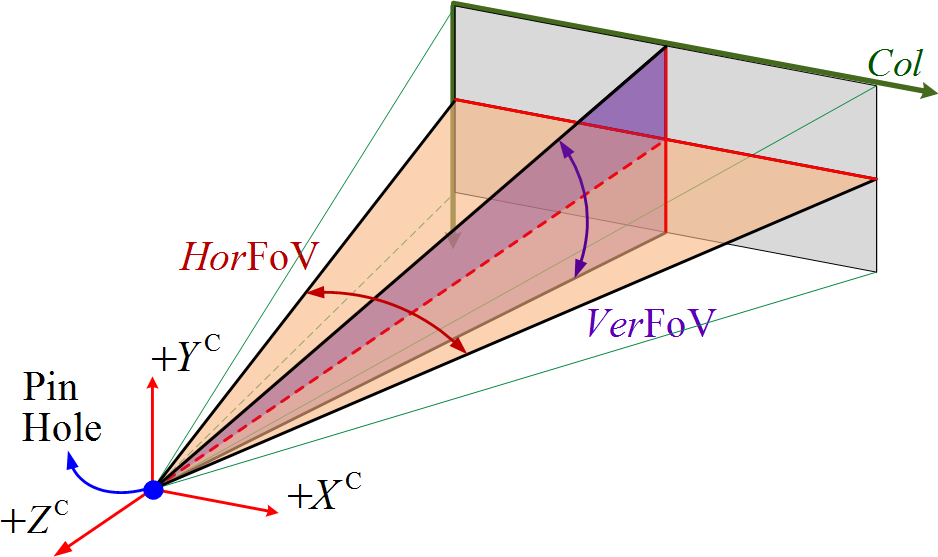
\includegraphics[width=0.7\textwidth]{VHfieldOfView}
\caption{Field of View in Pinhole-Camera Model}
\label{VHfieldOfView}
\end{figure}%
%
The \gls{KinectV2} depth sensor measures \(\gls{cameraZ}\) in millimeter and supports its positive data in unsigned-short data-type. Those data will be automatically converted into single-floating type with its range from 0.0f to +1.0f when uploaded onto \gls{GPU}. Considering that in practice \(\gls{D}\)s from \gls{KinectV2} are always positive whereas \(\gls{cameraZ}\)s should be always negative, we will add a negative sign in the un-scaling step to recover the \(\gls{cameraZ}\) in metric on \gls{GPU}:
\begin{equation}
\gls{cameraZ}[m, n] = - \beta \gls{D}[m, n] \, ,
\label{unscalingZc}
\end{equation}%
\noindent
where \(\beta\) constantly equals to 65535.0 (range of unsigned short in single-floating) for all pixels. Besides the depth stream, \gls{KinectV2} supports both of the horizontal and vertical field of view (\gls{FoV}) that can help generate per-pixel \(\gls{cameraX}\) and \(\gls{cameraY}\), which share the same credits with the intrinsic parameters in a pinhole camera model. Figure~\ref{VHfieldOfView} shows an intuitive view of the horizontal and vertical FoVs in a pinhole camera model, based on which we can derive the \(\gls{cameraX}\) and \(\gls{cameraY}\) values given a random \(\gls{cameraZ}\) value on the per-pixels basis. Assuming the depth sensor, with its size numDepthRows by numDepthCols, is observing right perpendicularly to a wall where all pixels share the same \(|\gls{cameraZ}_0|\) from the sensor to the wall. Talking about the horizontal \gls{FoV} only, it is easy to get the range of the camera space \gls{FoV} along 
\(\gls{cameraX}\)-axis from \(-|\gls{cameraX}_{\text{Max}}|\) to \(|\gls{cameraX}_{\text{Max}}|\), as shown in Fig.~\ref{horizontalFoVtoColumns}. %
\begin{figure}[!t]
\centering
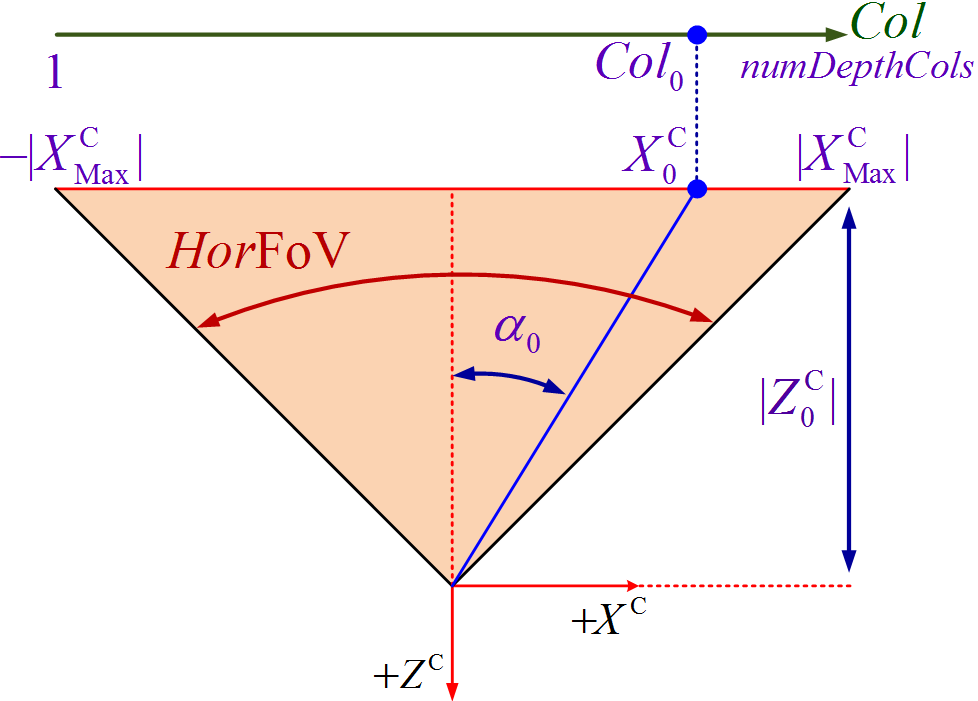
\includegraphics[width=0.6\textwidth]{horizontalFoVtoColumns}
\caption{map \(\gls{imageColumn}\) to \(\gls{cameraX}\) via horizontal \gls{FoV}}
\label{horizontalFoVtoColumns}
\end{figure}%
%
The horizontal range value \(|\gls{cameraX}_{\text{Max}}|\) depends on \(|\gls{cameraZ}_0|\) and the horizontal \gls{FoV}, given by:
%
\begin{equation}
|\gls{cameraX}_{\text{Max}}| = |\gls{cameraZ}_0| \cdot tan(horFov / 2) 
\label{cameraXMaxfromZ}
\end{equation}%
\noindent
where the pixel observing on \(\gls{cameraX} = |\gls{cameraX}_{\text{Max}}|\) has its column address of numDepthCols. Similarly, given a random pixel of column address \(Col_0\), its horizontal view \(\gls{cameraX}_0\) could be expressed based on its own horizontal view angle \(\alpha_0\):
%
\begin{equation}
|\gls{cameraX}_{0}| = |\gls{cameraZ}_0| \cdot tan(\alpha_0)  .
\label{alphaZeroHorFOV}
\end{equation}%
\noindent
To combine eqn.~(\ref{cameraXMaxfromZ}) and eqn.~(\ref{alphaZeroHorFOV}), we get
%
\begin{equation}
\frac{\gls{cameraX}_0}{|\gls{cameraX}_{\text{Max}}|} = \frac{tan(\alpha_0)}{tan(horFov / 2)} = \frac{Col_0}{numDepthCols/2} - 1\, ,
\label{alphaZeroHorFOV}
\end{equation}%
\noindent
which shows how to get the per-pixel \(\gls{cameraX}_0\) from \(|\gls{cameraX}_{\text{Max}}|\) based on its column address, while \(|\gls{cameraX}_{\text{Max}}|\) depends on the depth sensor's horizontal filed of view. It is intuitively better to change eqn.~(\ref{alphaZeroHorFOV}) a little by substituting \(|\gls{cameraX}_{\text{Max}}|\) with eqn.~(\ref{cameraXMaxfromZ}) such that we can get eqn.~(\ref{proportionalEqnFromZtoX}), a proportional per-pixel mapping based on the column addresses from \(\gls{cameraZ}\) to \(\gls{cameraX}\).
%
\begin{equation}
\gls{cameraX}[m, n] = tan(horFov / 2) \cdot (\frac{n}{numDepthCols/2} - 1) \cdot |\gls{cameraZ}[m, n]|\, ,
\label{proportionalEqnFromZtoX}
\end{equation}%
\noindent
where [\(m,n\)] is the discrete space \(\gls{imageRow}\) and \(\gls{imageColumn}\) coordinate of each pixel in the depth sensor. Similarly, we can also get the proportional per-pixel mapping from \(\gls{cameraZ}\) to \(\gls{cameraY}\), based on the vertical \gls{FoV} and row addresses:
%
\begin{equation}
\gls{cameraY}[m, n] = tan(verFov / 2) \cdot (\frac{m}{numDepthRows/2} - 1) \cdot |\gls{cameraZ}[m, n]| \  .
\label{proportionalEqnFromZtoY}
\end{equation}%
\noindent
Note that, \(horFov\) and \(verFov\) are constant during image processing, such that the mapping functions from per-pixel \(\gls{cameraZ}\) to per-pixel \(\gls{cameraX}/\gls{cameraY}\) totally depend on a pixel's address [\(m, n\)]. Therefore eqn.~(\ref{proportionalEqnFromZtoX}) and eqn.~(\ref{proportionalEqnFromZtoY}) could be expressed as 
%
\begin{equation}
\begin{aligned}
\gls{cameraX}[m, n] &= a[m, n] \cdot |\gls{cameraZ}[m, n]|
\\%
\gls{cameraY}[m, n] &= b[m, n] \cdot |\gls{cameraZ}[m, n]| 
\end{aligned}
\label{proportionalBeamEqn}
\end{equation}%
\noindent
where
%
\begin{equation}
\begin{aligned}
a[m, n] &= tan(horFov / 2) \cdot (\frac{n}{numDepthCols / 2} - 1)
\\%
b[m, n] &= tan(verFov / 2) \cdot (\frac{m}{numDepthRows / 2} - 1) \, \, .
\end{aligned}
\label{parametersABofProportional}
\end{equation}%
\\\indent
%
\begin{figure}[!t]
\centering
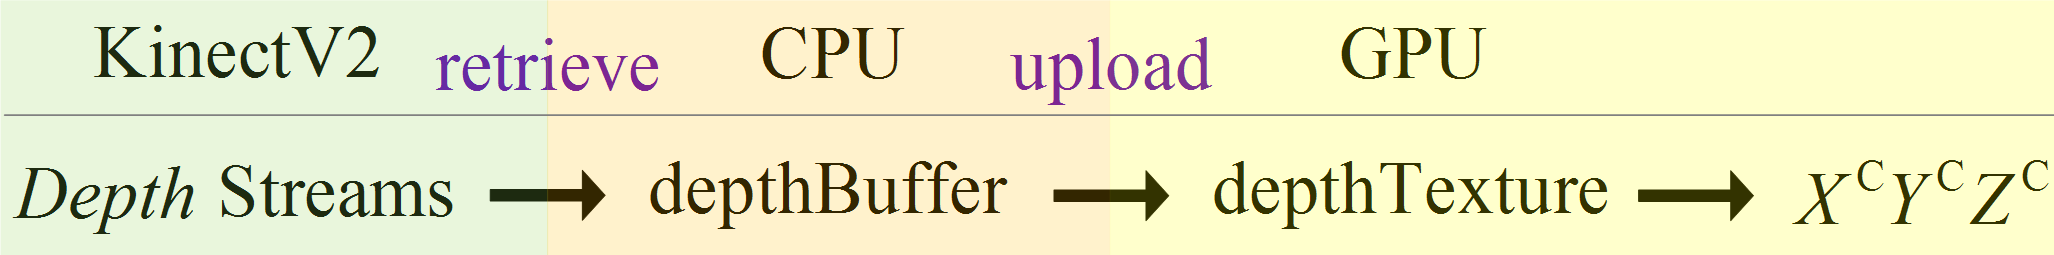
\includegraphics[width=0.8\textwidth]{cameraSpaceDiagram}
\caption{Diagram for Camera Space \gls{3D} Reconstruction without calibration}
\label{cameraSpaceDiagram}
\end{figure}%
%
Now that we have the per-pixel mapping from \(\gls{cameraZ}\) to \(X^CY^C\), it is time to draw the camera space \gls{3D} image on \gls{GPU}. Figure~\ref{cameraSpaceDiagram} shows the streams flow diagram. We will retrieve \(Depth\) streams from the \gls{KinectV2} camera, save them into corresponding buffers on CPU and upload the the streams onto \gls{GPU} as textures. Then the per-pixel's camera space \gls{3D} coordinates \(X^CY^CZ^C\) will be generated during its fragment-shader processing from depth texture based on eqn.~(\ref{proportionalBeamEqn}). The fragment shader is programmed as below.
\\%
{\ttfamily
\textbf{\textcolor[rgb]{0.5019608,0.5019608,0.0}{\ \ \ uniform }}\textcolor[rgb]{0.7529412,0.7529412,0.7529412}{
 }\textcolor[rgb]{0.5019608,0.5019608,0.0}{sampler2D }\textcolor[rgb]{0.7529412,0.7529412,0.7529412}{
}qt\_depthTexture;\textcolor[rgb]{0.7529412,0.7529412,0.7529412}{
\ \ }}

{\ttfamily
\textbf{\textcolor[rgb]{0.5019608,0.5019608,0.0}{uniform }}\textcolor[rgb]{0.7529412,0.7529412,0.7529412}{
 }\textcolor[rgb]{0.5019608,0.5019608,0.0}{sampler2D }\textcolor[rgb]{0.7529412,0.7529412,0.7529412}{
}qt\_spherTexture;\textcolor[rgb]{0.7529412,0.7529412,0.7529412}{ \ }}


\bigskip

{\ttfamily
\textbf{\textcolor[rgb]{0.5019608,0.5019608,0.0}{layout}}(\textbf{\textcolor[rgb]{0.5019608,0.5019608,0.0}{location } }\textcolor[rgb]{0.7529412,0.7529412,0.7529412}{
}=\textcolor[rgb]{0.7529412,0.7529412,0.7529412}{
}0,\textcolor[rgb]{0.7529412,0.7529412,0.7529412}{
}\textbf{\textcolor[rgb]{0.5019608,0.5019608,0.0}{index } }\textcolor[rgb]{0.7529412,0.7529412,0.7529412}{
}=\textcolor[rgb]{0.7529412,0.7529412,0.7529412}{
}0)\textcolor[rgb]{0.7529412,0.7529412,0.7529412}{
}\textbf{\textcolor[rgb]{0.5019608,0.5019608,0.0}{out } }\textcolor[rgb]{0.7529412,0.7529412,0.7529412}{
 }\textcolor[rgb]{0.5019608,0.5019608,0.0}{vec4 }\textcolor[rgb]{0.7529412,0.7529412,0.7529412}{
}qt\_fragColor;}

{\ttfamily
\textcolor[rgb]{0.5019608,0.5019608,0.0}{void }\textcolor[rgb]{0.7529412,0.7529412,0.7529412}{
}main()}

{\ttfamily
\{}

{\ttfamily
\textcolor[rgb]{0.7529412,0.7529412,0.7529412}{\ \ \ \  }\textcolor[rgb]{0.5019608,0.5019608,0.0}{ivec2 }\textcolor[rgb]{0.7529412,0.7529412,0.7529412}{
}textureCoordinate\textcolor[rgb]{0.7529412,0.7529412,0.7529412}{
}=\textcolor[rgb]{0.7529412,0.7529412,0.7529412}{
 }\textcolor[rgb]{0.5019608,0.5019608,0.0}{ivec2}(
 \textcolor[rgb]{0.5019608,0.0,0.5019608}{gl\_FragCoord}.x, \textcolor[rgb]{0.7529412,0.7529412,0.7529412}{
 }\textcolor[rgb]{0.5019608,0.0,0.5019608}{gl\_FragCoord}.y);}

\bigskip

{\ttfamily
\textcolor[rgb]{0.7529412,0.7529412,0.7529412}{\ \ \ \ }\textcolor[rgb]{0.5019608,0.5019608,0.0}{float}\textcolor[rgb]{0.7529412,0.7529412,0.7529412}{
}z\textcolor[rgb]{0.7529412,0.7529412,0.7529412}{
} = \textcolor[rgb]{0.7529412,0.7529412,0.7529412}{
}\textbf{\textcolor[rgb]{0.5019608,0.5019608,0.0}{texelFetch}}(qt\_depthTexture,\textcolor[rgb]{0.7529412,0.7529412,0.7529412}{
}textureCoordinate,\textcolor[rgb]{0.7529412,0.7529412,0.7529412}{
}\textcolor[rgb]{0.0,0.0,0.5019608}{0}).r
*\textcolor[rgb]{0.7529412,0.7529412,0.7529412}{
}\textcolor[rgb]{0.0,0.0,0.5019608}{65535.0};}

{\ttfamily
\textcolor[rgb]{0.7529412,0.7529412,0.7529412}{\ \ \ \ }\textcolor[rgb]{0.5019608,0.5019608,0.0}{vec4}\textcolor[rgb]{0.7529412,0.7529412,0.7529412}{
\ }a\textcolor[rgb]{0.7529412,0.7529412,0.7529412}{
} = \textcolor[rgb]{0.7529412,0.7529412,0.7529412}{
}\textbf{\textcolor[rgb]{0.5019608,0.5019608,0.0}{texelFetch}}(qt\_spherTexture,\textcolor[rgb]{0.7529412,0.7529412,0.7529412}{
}textureCoordinate,\textcolor[rgb]{0.7529412,0.7529412,0.7529412}{
}\textcolor[rgb]{0.0,0.0,0.5019608}{0});}


\bigskip

{\ttfamily
\textcolor[rgb]{0.7529412,0.7529412,0.7529412}{\ \ \ \ }qt\_fragColor.x\textcolor[rgb]{0.7529412,0.7529412,0.7529412}{
} = \textcolor[rgb]{0.7529412,0.7529412,0.7529412}{
}{}-z\textcolor[rgb]{0.7529412,0.7529412,0.7529412}{
}*\textcolor[rgb]{0.7529412,0.7529412,0.7529412}{ }a.r;}

{\ttfamily
\textcolor[rgb]{0.7529412,0.7529412,0.7529412}{\ \ \ \ }qt\_fragColor.y\textcolor[rgb]{0.7529412,0.7529412,0.7529412}{
} = \textcolor[rgb]{0.7529412,0.7529412,0.7529412}{
}{}-z\textcolor[rgb]{0.7529412,0.7529412,0.7529412}{
}*\textcolor[rgb]{0.7529412,0.7529412,0.7529412}{ }a.g;}

{\ttfamily
\textcolor[rgb]{0.7529412,0.7529412,0.7529412}{\ \ \ \ }qt\_fragColor.z\textcolor[rgb]{0.7529412,0.7529412,0.7529412}{
} = \textcolor[rgb]{0.7529412,0.7529412,0.7529412}{ }{}-z;}

{\ttfamily
\}}

%
The uniform \emph{qt\_spherTexture} is a \(\gls{cameraZ}\) to \(\gls{cameraX}/\gls{cameraY}\) proportional mapping texture, which contains the per-pixel parameters \(a/b\) based on eqn.~(\ref{parametersABofProportional}). Note that we add three negative signs in front of \(X^CY^CZ^C\) respectively to account for the pinhole-imaging. %
%
\begin{figure}[t]
\centering
\subfloat[Front View][Front View]{
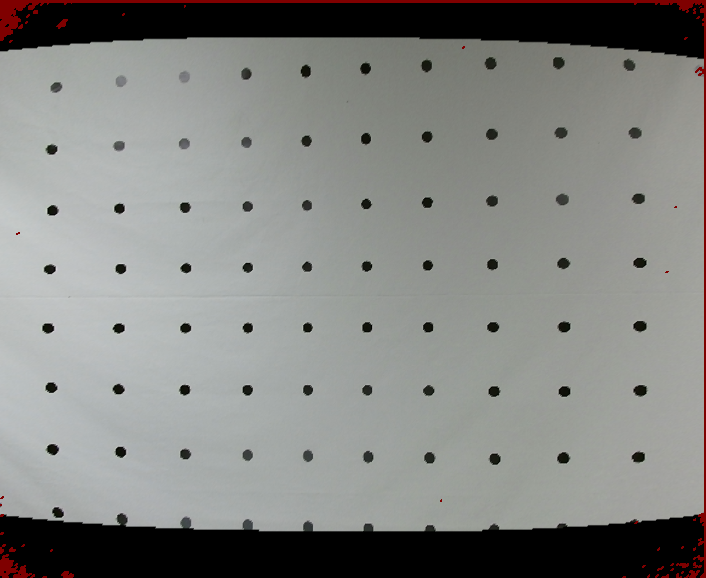
\includegraphics[height=0.42\textwidth]{distortedRGB}
\label{distortedRGB}}
\subfloat[Left View][Left View]{
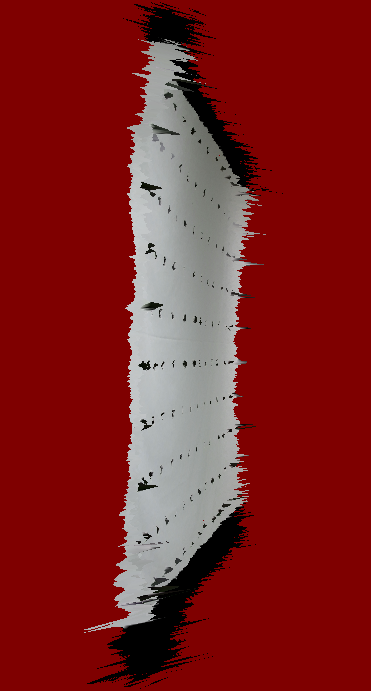
\includegraphics[height=0.42\textwidth , width = 0.4\textwidth]{distortedSideViewRGB}
\label{distortedSideViewRGB}}
%\qquad
\caption{Colored Camera Space \gls{3D} Reconstruction}
\label{reconstructionInCameraSpace}
\end{figure}%
%
The whole parallel image processing above shows a natural \gls{3D} reconstruction on \gls{GPU}. Figure~\ref{reconstructionInCameraSpace} shows the view of camera space \gls{3D} reconstruction when observing uniform grid dots pattern on the flat wall. We can tell from the image that, this reconstruction is totally based on raw data, without calibration at all. Not only the \(X^CY^C\) plane is apparently deformed (lens distortions) in the front view, but the \(\gls{cameraZ}\) is also not as flat as it should be, which we will call it \emph{depth distortion} since now. The \emph{depth distortion} comes from the imperfect depth resolutions among pixels, \textit{i.e.}, \(\gls{cameraZ}_{[row, col]} - Depth_{[row, col]} \neq E_{\text{Constant}}\), which lead to bumps and hollows in the camera space reconstruction when observing a flat wall. Therefore, a per-pixel calibration is necessary for an undistorted \gls{3D} image.

%%%%%%%%%%%%%%%%%%%%%%%%%%%%%%%%%%%%%%%%%%%%%%%%%%%%%%%%%%%%%%%%%%%%%%%%%%%%%%%%%%%%%%%%%%%%%%%%%%%%%%%%%%%%%%%%%%%%%%%%%%%%%%%%%%%%%%%%%%%%%%%%%%%%%%%%%%%%%%%%%%%%%%%%%%%%%%%%%%%%%%%%%%%%%%%%%%%%%%%%%%%%%%%%%%%%%%%%%%%%%%%%%%%%%%%%%%%%%%%%%%%%%%%%%%%%%%%%%%%%%%%%%%%%%%
\section{Rail Calibration System}
\label{sectionRailCalibrationSystem}
Talking about camera calibration, the pinhole camera matrix \(M\) will come up in most people's mind. As discussed in Chapter~\ref{chapterTraditionalCalibration}, the pinhole-camera matrix \(M\) consists of an intrinsic matrix \(K\) and an extrinsic matrix \([R_{3*3}, T_{3*1}]\). The camera space \gls{3D} reconstruction method we discussed in section~\ref{sectionCameraSpaceReconstruction} utilizes horizontal and vertical field of view (\gls{FoV})s, which works in the same way with the intrinsic matrix \(K\)'s principle. However, a camera's calibration needs external help from world space objects, which means neither of the FoVs nor intrinsic matrix \(K\) alone is able to do calibration,  and extrinsic parameters that can link to world space are necessary in calibration. 
\\\indent
Kai \cite{Kai10} did a good job on structured light \gls{3D} scanner parallel calibration on \gls{GPU}, and derived the per-pixel beam equation~(\ref{kaiBeamEquationCh3}) directly from a pinhole camera matrix \(M\), which offers the possibility of natural \gls{3D} reconstruction on \gls{GPU} similar to eqn.~(\ref{proportionalBeamEqn}).
%
\begin{equation}
\begin{aligned}
\gls{worldX}[m,\,  n] = a[m, n]\gls{worldZ}[m,\,  n]+b[m, n]
\\%
\gls{worldY}[m,\,  n] = c[m, n]\gls{worldZ}[m,\,  n]+d[m, n]
\end{aligned} \ ,
\label{kaiBeamEquationCh3}
\end{equation}%
\noindent
where [\(m,n\)] is the discrete space \(\gls{imageRow}\) and \(\gls{imageColumn}\) coordinate of each pixel in a M by N sensor. This per-pixel beam equation shows per-pixel linear mappings from \(\gls{worldZ}\) to \(\gls{worldX}/\gls{worldY}\), and the per-pixel \(\gls{worldZ}\) can be mapped from features of structured light. It is not specially proportional like eqn.~(\ref{proportionalBeamEqn}), because it contains space translation infos from camera space to world space. Although it is in world space now and the intrinsic parameters are able to be determined, however, lens distortions are still not able to be handled. To make it ideal, we need to not only remove the lens distortions and \emph{depth distortion}, but also realize the \gls{3D} reconstruction on \gls{GPU} in a natural method similar to eqn.~(\ref{kaiBeamEquationCh3}).
\\\indent
%
In this section, we will find a best-fit calibration system for a \gls{KinectV2} camera's natural calibration and reconstruction, which is able the handle both of lens distortion and \emph{depth distortion}. %
%The \gls{KinectV2} camera has one depth sensor and one RGB sensor. The RGB sensor offers RGB streams, whose color infos will be aligned to pixels according to their corresponding world space coordinates after the \gls{3D} reconstruction. The depth sensor offers \gls{NearIR} and Depth streams, both of which share the same size ($row$ and $column$) and lens distortions of the depth sensor, and can both be utilized for lens distortion correction. We will use the Depth stream to recover world space \gls{3D} coordinates $X^WY^WZ^W$ for reconstruction, during which the \gls{NearIR} stream will be used for lens distortion correction. 
%\\\indent
To easily show \gls{3D} reconstruction in a parallel way on the \gls{GPU}, we would like our calibration system to be able to offer a per-pixel mapping from \(\gls{D}\) to \(\gls{worldZ}\), which then could be used to map to \(\gls{worldX}/\gls{worldY}\) using eqn.~(\ref{kaiBeamEquationCh3}). In this way, the \emph{depth distortion} could also be corrected during the per-pixel \(\gls{D}\) to \(\gls{worldZ}\) mapping. Of all different kinds of calibration systems, a camera on rail system with a planar pattern on wall is finally decided, which offers a moving plane with respect to the camera when the camera moves along the rail. As Fig.~\ref{trackingModuleOnKinectV2CalibrationSystemCh3} shows, a canvas on which printed an uniform grid dots pattern is hung on the wall, and the rail is required to be perpendicular to the wall. 
%
\begin{figure}[t]
\centering
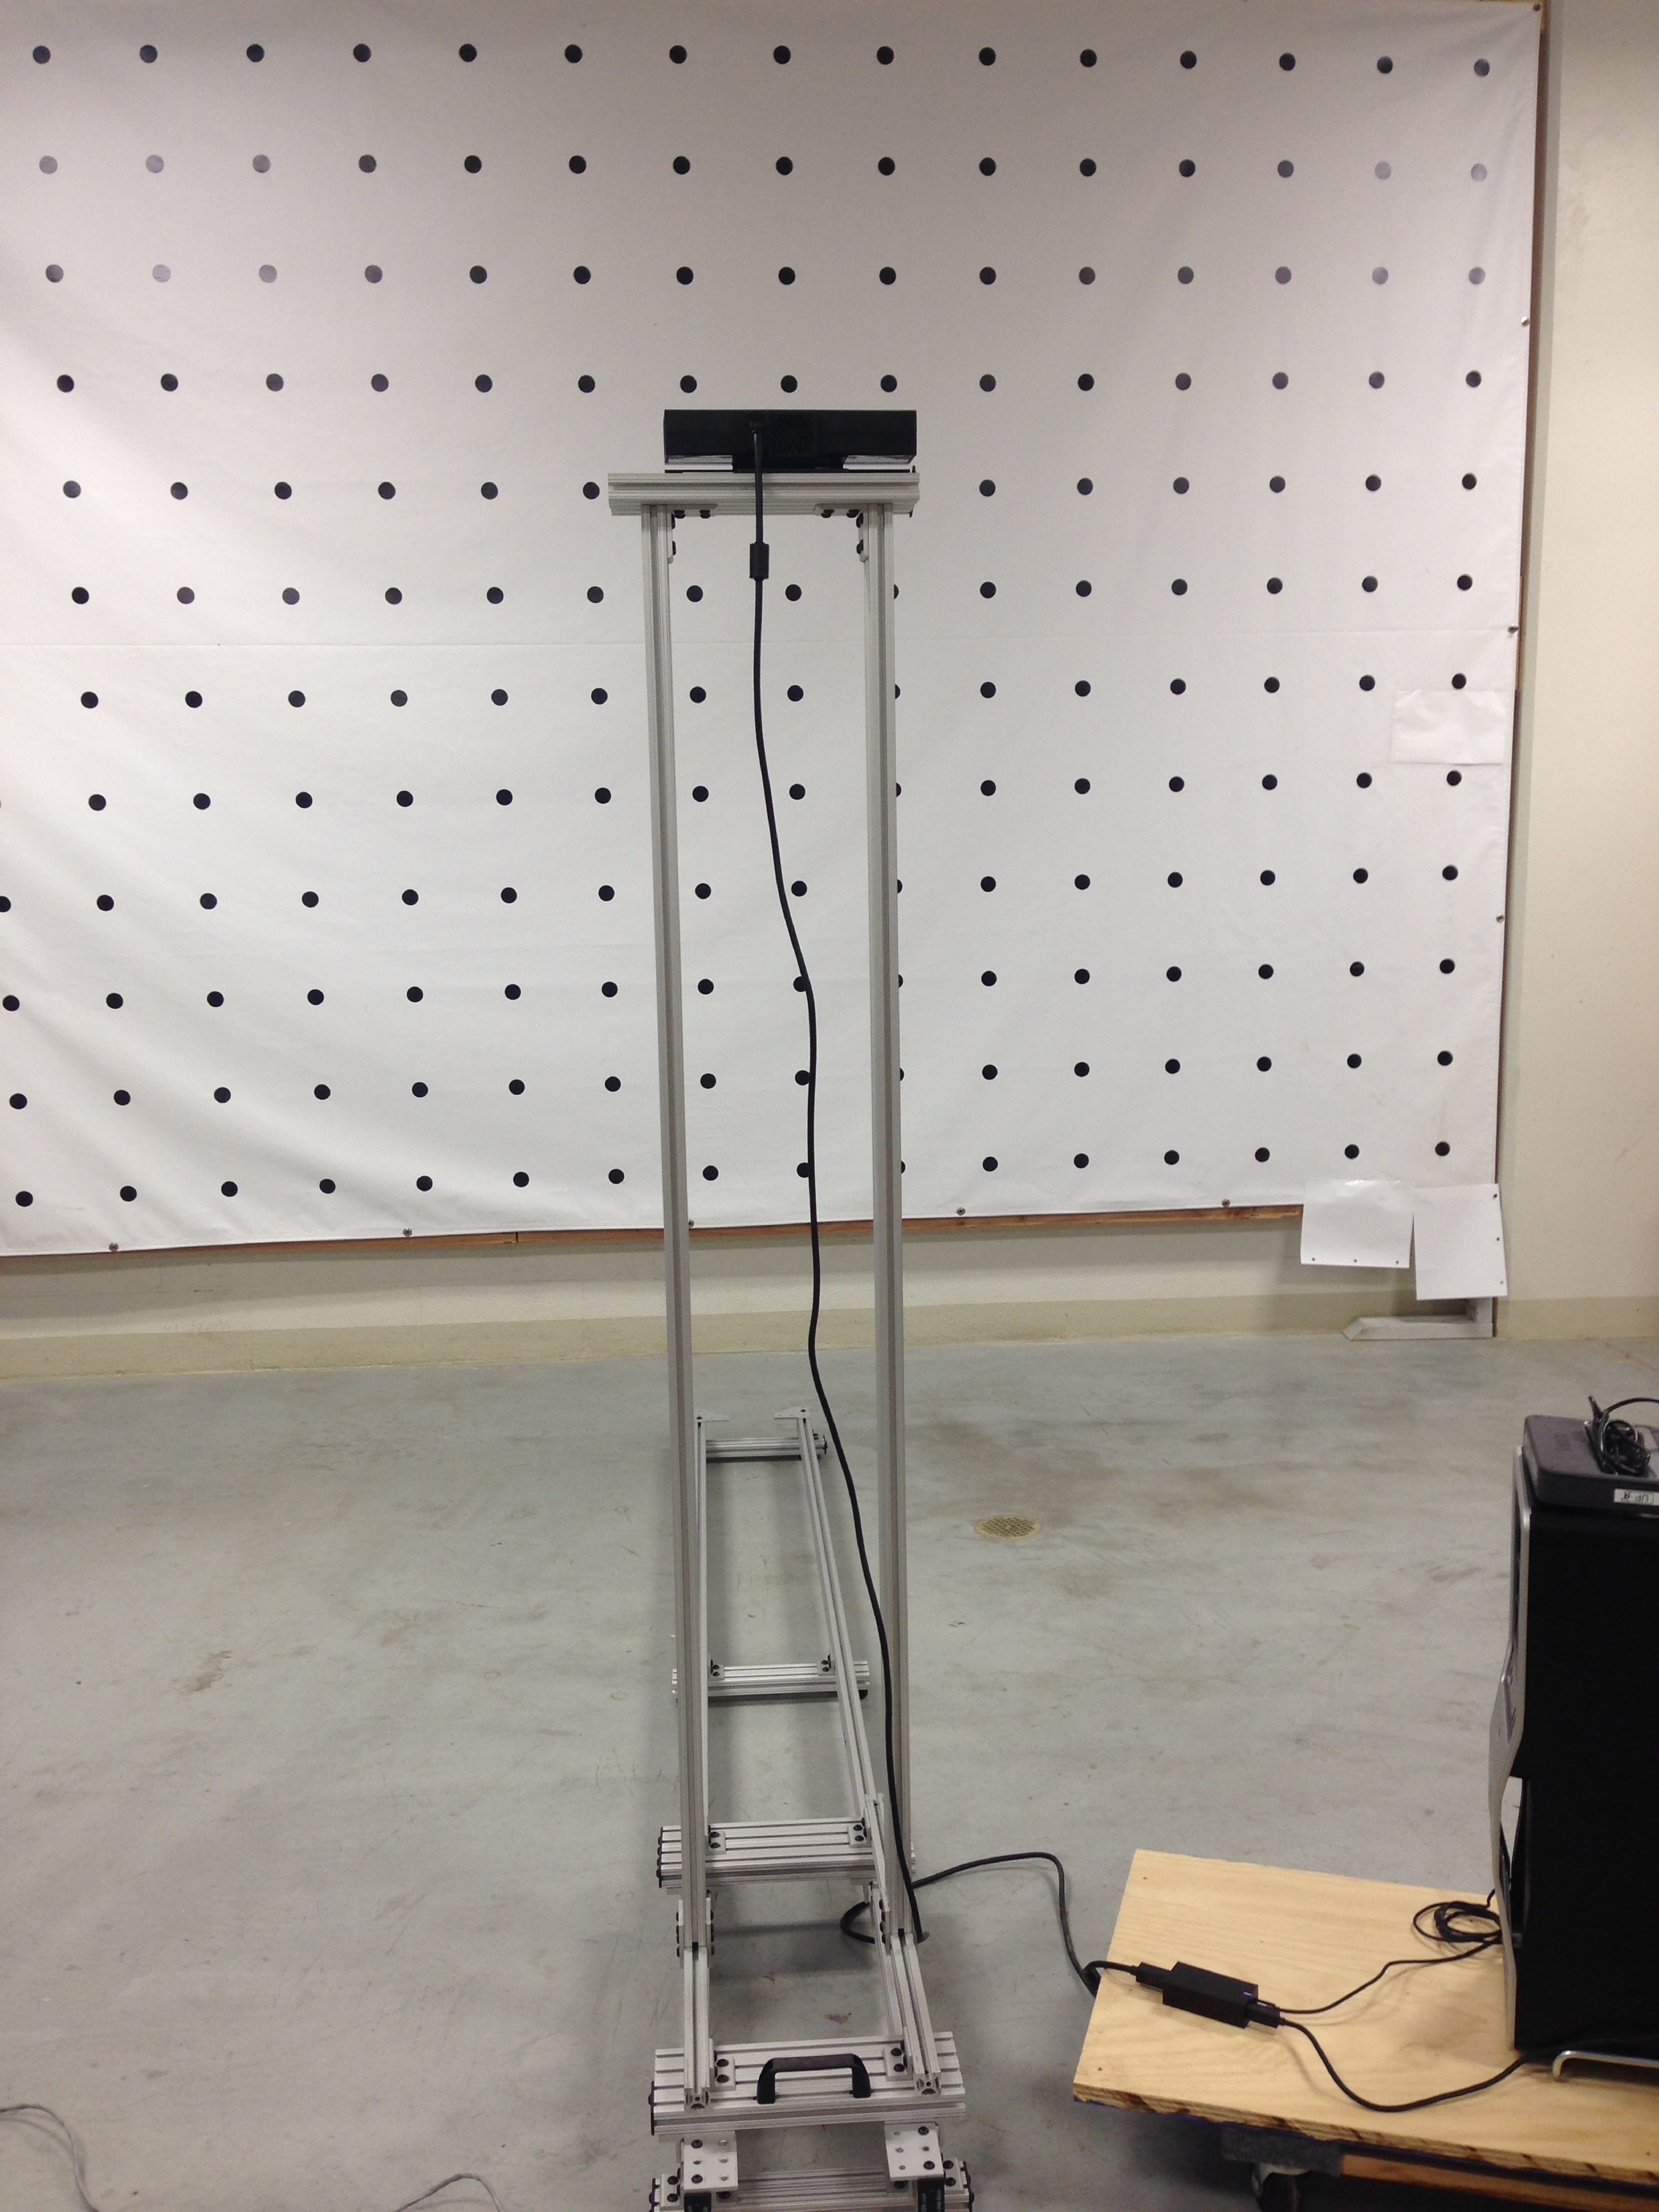
\includegraphics[width=0.55\textwidth]{trackingModuleOnKinectV2CalibrationSystem}
\caption{\gls{KinectV2} Calibration System}
\label{trackingModuleOnKinectV2CalibrationSystemCh3}
\end{figure}%
%
The \gls{RGBD} camera waiting to calibrate is mounted on the slider. Note that, in this calibration system, the only unit that needs to be perpendicular to the wall is the rail, whereas the \gls{RGBD} camera has no need to require its observation orientation. Because the per-pixel calibration requires only accurate world space coordinates which will be decided by the rail and the wall, whereas the camera's space is not considered at all. We will assign the pattern plane as the \(X^WY^W\) plane in world space, and the rail to be along with (not exactly on) \(\gls{worldZ}\)-axis. The world coordinate is static with the camera on the slider. %
%
%
\\\indent
\begin{figure}[!t]
\centering
%calibrated \(X^{W}\)/\(Y^{W}\) and \(Z^{W}\)
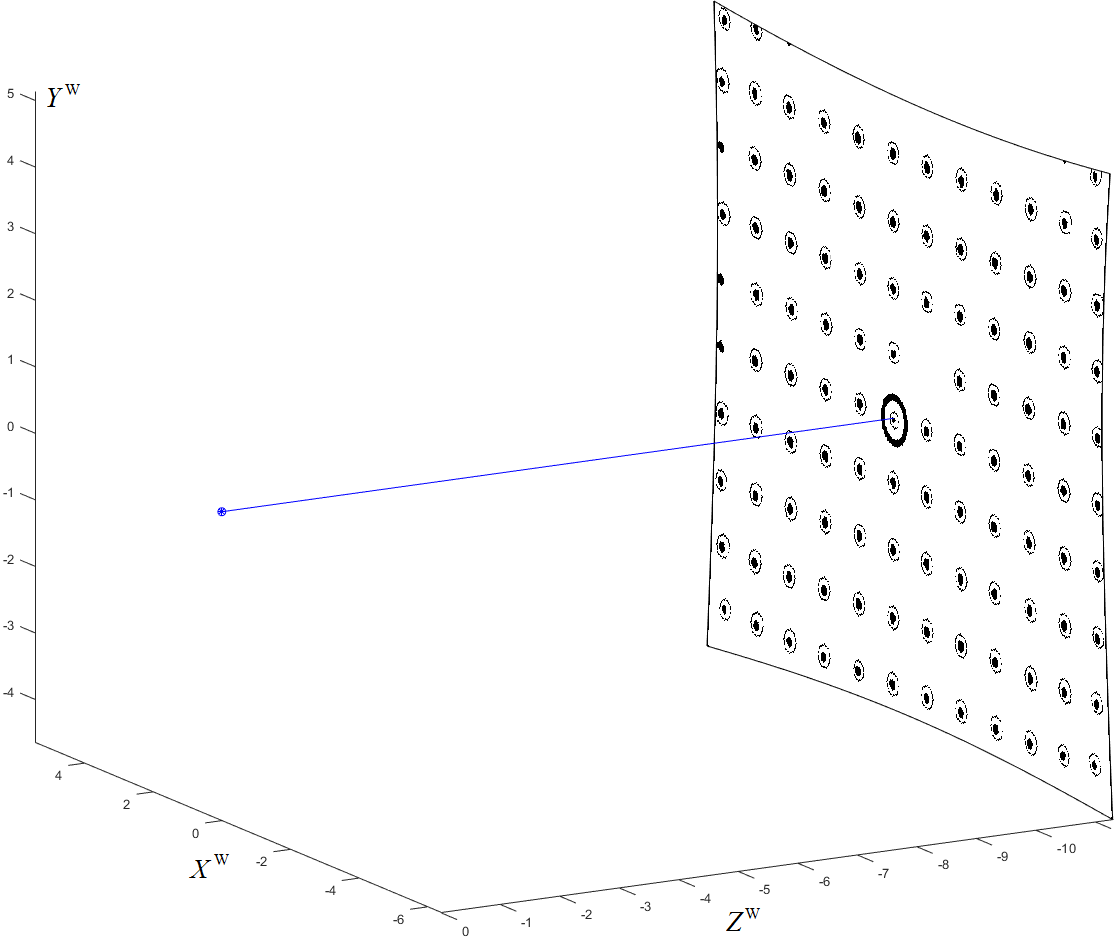
\includegraphics[width=0.7\textwidth, height= 0.5\textwidth]{OneFrameXYZ_Calibrated}
\caption{\gls{NearIR} \(X^{W}Y^{W}Z^{W}\) \gls{3D} Reconstruction}
\label{OneFrameXYZ_Calibrated}
\end{figure}%
%
Figure~\ref{OneFrameXYZ_Calibrated} shows one frame of \gls{NearIR} \(X^WY^WZ^W\) \gls{3D} reconstruction, which can help a lot explaining how the world space origin is assigned. Inside the figure, both of the origin and \(Z\)-axis are high-lighted in blue, and the origin of world space is on the left end of the blue line. On the pattern plane with dot-clusters marked in circles, we can see one dot-cluster is high-lighted inside a thick circle, and its center point is where \(\gls{worldX}/\gls{worldY} = 0\). The dot-cluster which will be sitting on the \(\gls{worldZ}\)-axis is the one whose center point is closest to the center pixel of the sensor. All pixels in this frame share the exact same \(\gls{worldZ}\), which is also why we require the rail to be perpendicular to the pattern. And the value of \(\gls{worldZ}\) is measured by a laser distance measurer that static with the camera. The final origin of the world space will be decided by both of the camera's observing orientation and the laser distance measurer's position. This kind of world coordinate assignment is totally for simplifying image processing during calibration.  Practically, we do not even care where exactly the origin is, as long as the rail is perpendicular to the pattern and the distance measurer is static with the camera.
\\\indent
With this rail calibration system, infinite number of frames with infinite number of calibration points could be utilized for training a calibration model. Besides, as the slider moves along the rail, the amount and distribution of the grid dots captured by the camera will change, which means a dynamic pattern for calibration instead of static. With more and more dots walking into the camera's field of view under a certain rhythm as the slider moves further from the pattern plane, the dots (which will be extracted as calibration points) are able to cover all pixels of a sensor. What's more, a moving-plane system (multiple frames calibration instead of one frame calibration) makes it possible to do dense \(\gls{D}\) to \(\gls{worldZ}\) mapping, which will handle \emph{depth distortion}.


\section{Data Collection}
\label{perpixelDataCollection}
%
With the calibration system built up and world coordinate assigned, we are now ready to calibrate. \(Z^{W}\) values for all pixels of every frame will be supported from external laser distance measurer. To simplify potential calculation during image processing, we assign the world coordinate \emph{Unit One} based on the uniform grid dots patter, to be same with the side of pattern's unit-square. Concretely, the distance between every two adjacent dots' centers in real-world is 228mm. Therefore, \(Z^{W}\) = -\(Z\)(mm) / 228(mm), where \(Z\) is the vertical distance to the pattern plane in reality measured by the laser distance measurer. Note that, \(Z^{W}\) values are always negative, based on the assignment of Cartesian world coordinate. The outline of calibration procedures is listed below.
%
\begin{enumerate}
   	\item Mount both of the camera and laser distance measurer onto the slider.
   	\item Move the slider to the nearest position to the pattern plane.
   	\item Record one frame of RGB data with one frame of \gls{NearIR} data at this position.
   	\label{repeatMovingSlider}
   	\begin{enumerate}
     		\item measure \(|\gls{worldZ}|\) using the laser distance measurer.
     		\item grab RGB, \gls{NearIR} and Depth streams from \gls{KinectV2} camera.
     		\item extract center points (\(R/C\)) of dot-clusters from RGB and \gls{NearIR} streams respectively.
     		\item assign \(\gls{worldX}/\gls{worldY}\) values to the extracted points, RGB and \gls{NearIR} respectively.
     		\item train and determine the best-fit high order polynomial model that map from \(RC\) to \(\gls{worldX}/\gls{worldY}\), RGB and \gls{NearIR} respectively.
     		\item generate dense \(\gls{worldX}/\gls{worldY}\) for all pixels using the model, for \gls{NearIR} and RGB streams respectively.
     		\item save 2 frames of RGB and \gls{NearIR} all pixels' data respectively: \(X^WY^WZ^WRGBD\) for RGB stream, and \(X^WY^WZ^WID\) for \gls{NearIR} stream, where the channel \(I\) in \gls{NearIR} frame denotes \emph{Intensity}.
   	\end{enumerate}
	\item Move the slider to the next position, and repeat step~\ref{repeatMovingSlider}.
%	\item Check all \(\gls{worldX}/\gls{worldY}\) values of all frames, unify the staggered origin by adding or subtracting a corresponding integer (make sure the point \(X^WY^W = 0\) is at the same dot-cluster for all frames).
%	\item Determine the per-pixel mapping from \(\gls{D}\) to \(\gls{worldZ}\) and from \(\gls{worldZ}\) to \(\gls{worldX}/\gls{worldY}\) for all pixels using the \gls{NearIR} frames of data, and generate a \(\gls{imageRow}\)-by-\(\gls{imageColumn}\)-by-6 look-up table.
%	\item Determine a pinhole-camera matrix that can map \(\gls{worldX}/\gls{worldY}/\gls{worldZ}\) to \(R/C\) using RGB frames of data (for the RGB values' alignment to pixels after \gls{3D} reconstruction).
\end{enumerate}
%
Concretely, we will record RGB and \gls{NearIR} frames every 25mm at a time. During every time, \(|\gls{worldZ}|\) will be measured by the laser measurer and manually input into the shader at the very beginning of streams recording. After RGB, \gls{NearIR} and Depth streams have been retrieved from \gls{KinectV2}, we will utilize digital image processing (\gls{DIP}) techniques to extract the center points' image addresses (\(R/C\)) of dot-clusters, and then determine a high-order polynomial model to build a mapping from \(RC\) to \(\gls{worldX}/\gls{worldY}\) for dense world coordinates generation.

\subsection{\gls{DIP} Techniques on (\(R,\, C\)) Extraction}
\label{sectionDIPTechniques}
%  add noises analysis
\indent
A robust \gls{DIP} process on the extraction the points' addresses (\(R,\, C\))s determines the accuracy of calibration. In this project, the extraction steps consist of gray-scaling, histogram equalization, adaptive thresholding and a little trick on black pixels counting. OpenGL is selected as the \gls{GPU} image processing language. The default data type of steams saved on \gls{GPU} during processing is single-floating, with a range from 0 (balck) to 1 (white). 
\\\indent
Gray-scaling is done to unify processing steps of both RGB and \gls{NearIR} steams. For \gls{NearIR} steam, its data contains only color gray and data will be saved on \gls{GPU} as single-floating automatically. Whereas for RGB steam, a conversion from RGB to gray value is needed. Typically, there are three converting methods: lightness, average, and luminosity. The luminosity method is finally chosen as a human-friendly way for gray-scaling, give by
%
\begin{equation}
Intensity_{\text{\_gray}} =  0.21 Red\,  + \, 0.72 Green \, + \, 0.07 Blue  \, \, ,
\label{luminosityGrayScaling}
\end{equation}%
which uses a weighted average value to account for human perception.
\\\indent%
The pixel intensity values are automatically converted into single-floating type with its range from 0.0f to 1.0f, where \enquote{0.0f} means 100\% black and \enquote{1.0f}  means 100\% white. In practice, \gls{NearIR} steam image is always very dark, as shown in Fig.~\ref{Raw_Single_NIR} (with their intensity values every close to zero).  In order to enhance the contrast of \gls{NearIR} image for a better binarizing, histogram equalization technique is utilized to maximize the range of valid pixel intensity distributions. Same process is also compatible on the RGB stream.
%
 \begin{figure}[t]
\hspace*{-0.5cm}
\centering
\subfloat[Raw \gls{NearIR}][Raw]{
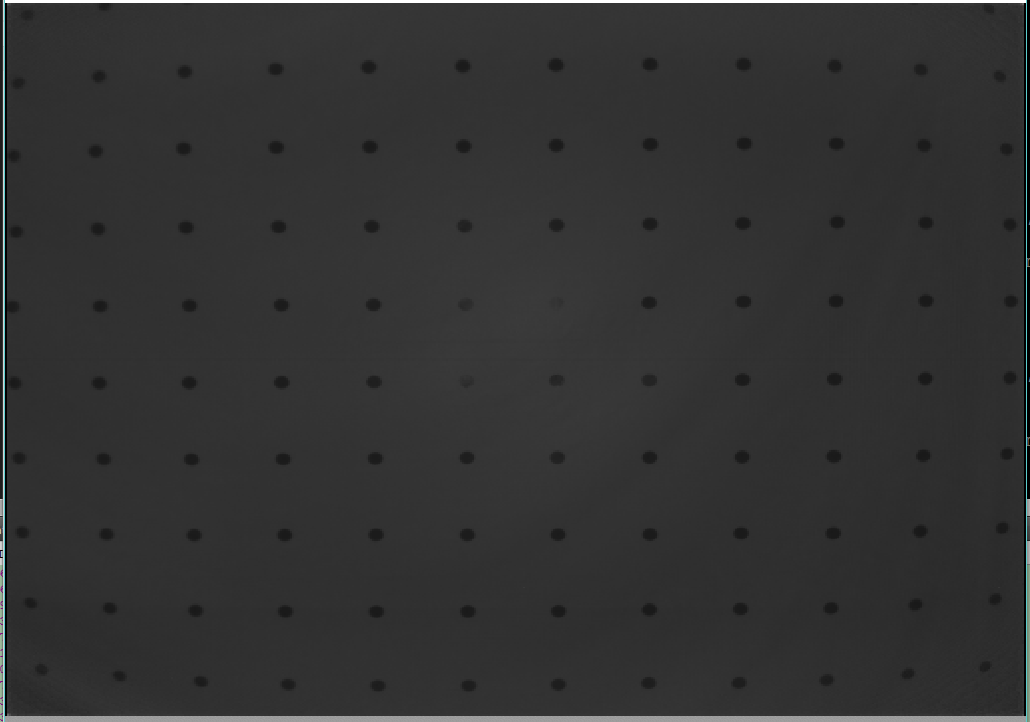
\includegraphics[width=0.5\textwidth]{Raw_Single_NIR}
\label{Raw_Single_NIR}}
\subfloat[Histogram Equalized \gls{NearIR}][Histogram Equalized]{
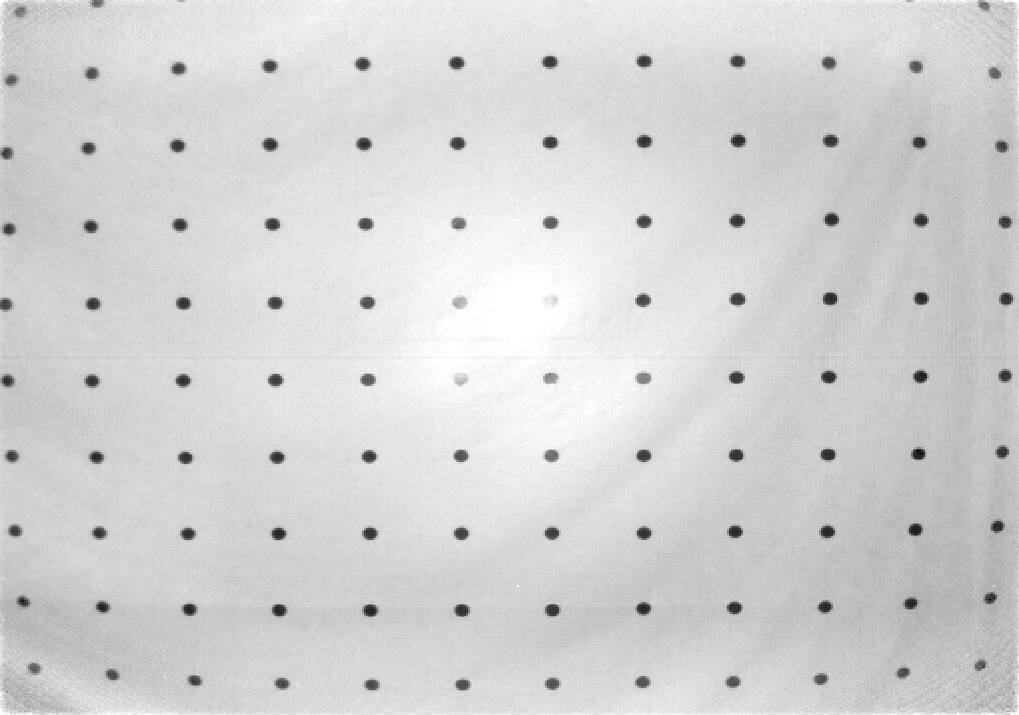
\includegraphics[width = 0.5\textwidth]{NIR_After_HistogramEqualization}
\label{NIR_After_HistogramEqualization}}
%\qquad
\caption{\gls{NearIR} Streams before / after Histogram Equalization}
\label{Histogram_Equalization}
\end{figure}%
%
Commonly, Probability Mass Function (PMF) and Cumulative Distributive Function (CDF) will be calculated to determine the minimum valid intensity value (\(floor\)) and maximum valid value (\(ceiling\)) for rescaling, whereas tricks could be used by taking advantage of the \gls{GPU} drawing properties.%
\\\indent%
PMF means the frequency of every valid intensity value for all of the pixels in an image. The calculation of PMF on \gls{GPU} will be very similar to points' drawing process, both of which are on a per-pixel basis. Dividing all of the pixels in terms of their intensity values into \(N\) levels, every pixel belongs to one level of them, which is called gray level. With a proper selection of \(N\) to make sure a good accuracy, the intensity value of a pixel could be expressed based on its gray level \(n\)
%
\begin{equation}
Intensity = n/N * (1.0f - 0.0f) + 0.0f = n/N \, ,
\end{equation}%
\noindent
where \(n\) and \(N\) are integers and \(1 \leqslant n \leqslant N\). We will count PMF by drawing all pixels with \enquote{1} being their intensity (color) value, zero being \(y\)-axis all the time and their original intensity being their position on \(x\)-axis. Thus, PMF values at various gray levels could be drawn into a framebuffer object.
\\\indent%
With PMF determined, CDF at gray leverl \(n\) could be calculated by
%
\begin{equation}
CDF(n) = \frac{sum}{N_{\text{\_Num of Total Pixels}}} \, ,
%\label{lensDistortion}
\end{equation}%
%
where \(sum\) denotes the summation of PMF added up consecutively from gray leverl 1 till \(n\), and \(N\) denotes how may pixels totally in a image. %
%
Then, the intensities \(floor\) and \(ceiling\) could be determined by 
%
\begin{equation}
\begin{aligned}
floor &=  n_{\text{\_floor}} / N%
\\%
ceiling &=  n_{\text{\_ceiling}} / N 
\end{aligned}
\label{intensityFloorCeilingDetermination}
\end{equation}%
through choosing appropriate CDFs, e.g., \(CDF(n_{\text{\_floor}}) = 0.01\) and \(CDF(n_{\text{\_ceiling}}) = 0.99\). Finally, a new intensity value of every single pixel in an image could be rescaled by
%
\begin{equation}
Intensity_{\text{\_new}} = \frac{Intensity_{\text{\_original}} - floor}{ceiling - floor} \, ,
\end{equation}%
%
\noindent
and the image will get a better contrast, as compared in Fig.~\ref{Histogram_Equalization}.%
\\\indent%
%% Adaptive Thresholding
Affected by radial dominated lens distortions, the intensity value tend to decrease as the position of a pixel moves from the center of an image to the borders, in the case of observing a singular color view. Therefore, an adaptive thresholding process is needed, whereas using fixed thresholding will generate too much noise around borders. To segment the black dots from white background, we could simply subtract an image's background from an textured image, where the background comes from a blurring process of that image.%
%
There are three common types of blurring filters: mean filter, weighted average filter, and gaussian filter. Mean filter is selected for this background-aimed blurring process, because it has the smallest calculation and also a better effect of averaging than the others. After the blurred image containing background information is obtained, the binarizing (subtraction) process for every single pixel could be written as
%
\begin{equation}
%
Intensity_{\text{\_binarized}} = %
%
\begin{cases}
\,\, 1 , \quad \quad I_{\text{\_textured}} - I_{\text{\_background}}  -  C_{\text{\_offset}} \,\, > \,\,0 %
\\%
\,\, 0 , \quad \quad \quad \quad else%
\end{cases}
 \, ,%
\end{equation}%
%
where \(I\) is short for \(Intensity\) of every single pixel, and \(C_{\text{\_offset}}\) is a small constant that could be adjusted depending on various thresholding situations. In this project, \(C_{\text{\_offset}}\) is around 0.1.%
%
\begin{figure}[t]
\hspace*{-0.5cm}
\centering
\subfloat[Histogram Equalized \gls{NearIR}][Histogram Equalized]{
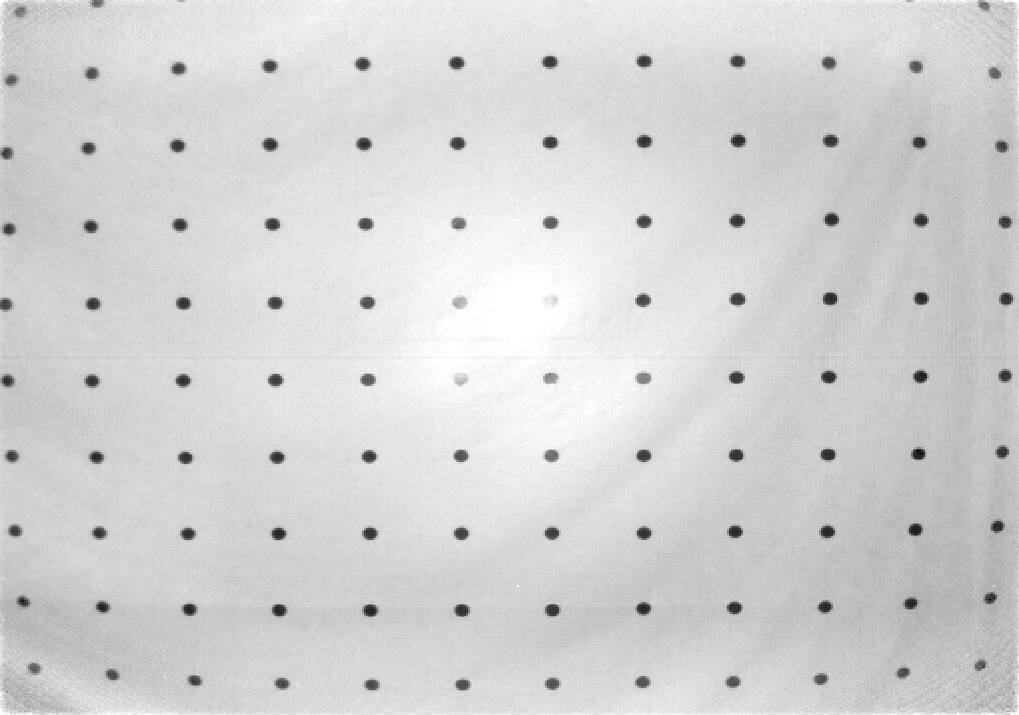
\includegraphics[width = 0.5\textwidth]{NIR_After_HistogramEqualization}
\label{NIR_After_HistogramEqualization_2}}
\subfloat[After Adaptive Thresholding][Binarized]{
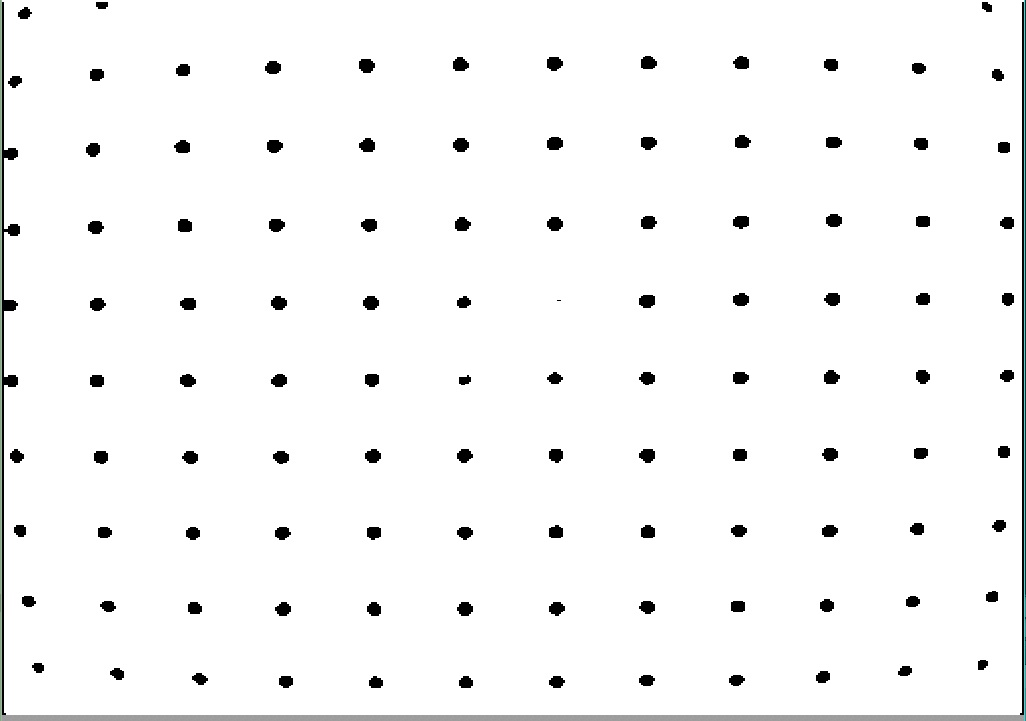
\includegraphics[width=0.5\textwidth]{Binarized_Single_NIR}
\label{Binarized_Single_NIR}}%\qquad
\caption{\gls{NearIR} Streams before / after Adaptive Thresholding}
\label{Adaptive_Thresholding}
\end{figure}%
%%
To sharpen the edge of the binarized image for a better \enquote{circle} shape detection, a median filter could be added as the last step of adaptive thresholding. As shown in Fig.~\ref{Adaptive_Thresholding}, background is removed in the binarized image after adaptive thresholding.
\\\indent
%
%
% Sniffer for Round Dot Center
After the adaptive thresholding, image data saved on \gls{GPU} is now composed of circle-shaped \enquote{0}s within a background of \enquote{1}s. In order to locate the center of those \enquote{0}s circle, which is the center of captured round dot, it is necessary to know the edge of those circles. A trick is used to turn all of the edge data into markers that could lead a pathfinder to retrieve circle information.%
%
The idea that helps to mark edge data is to reassign pixels' values (intensity values) based on their surroundings. Using letter \(O\) to represent one single pixel in the center of a $3\times3$ pixels environment, and letters from \(A\)\texttildelow \(H\) to represent surroundings, a mask of 9 cells for pixel value reassignment could be expressed as below.

\begin{center}
  \begin{tabular}{ | c | c | c | }
    \hline
    \(E\) & \(A\) & \(F\) \\ \hline
    \(B\) & \(O\) & \(C\) \\ \hline
    \(G\) & \(\gls{D}\) & \(H\) \\
    \hline
  \end{tabular}
\end{center}
%
To turn the surroundings \(A\)\texttildelow \(H\) into marks, different weights will be assigned to them. Those markers with different weights have to be non-zero data, and should be counted as the edge-part of circles. Therefore, the first step is to inverse the binary image, generating an image that consists of circle-shaped \enquote{1}s distributed in a background of \enquote{0}s.%
%
After reversing, the next step is to assign weight to the surroundings. OpenGL offers convenient automatic data type conversion, which means the intensity values from \enquote{0} to \enquote{1} of single-floating data type save on \gls{GPU} could be retrieved to CPU as unsigned-byte data type from \enquote{0} to \enquote{255}. Considering a bitwise employment of markers, a binary calculation related weight assignment is used in the shader process for pixels. The intensity reassignment for every single pixel is expressed as the equation below.
%
\begin{equation}
\hspace*{-0.1cm}%
%
I_{\text{\_Path Marked}} = I_{\text{\_Original}} * \frac{(128I_{\text{A}} + 64I_{\text{B}} + 32I_{\text{C}} + 16I_{\text{\gls{D}}} + 8I_{\text{E}} +  4I_{\text{F}} +  2I_{\text{G}}+I_{\text{H}})}{ 255 }
%
\label{snifferDistributionWeight}
\end{equation}%
\indent%
After this reassignment, the image is not binary any more. Every non-zero intensity value contains marked information of its surroundings, data at the edge of circles are now turned into fractions. In other words, the image data saved on \gls{GPU} at the moment is composed of \enquote{0}s as background and \enquote{non-zero}s circles, which contains fractions at the edge and \enquote{1}s in the center.%
%
Now, it is time to discover dots through an inspection over the whole path-marked image, row by row and pixel by pixel. Considering that, a process of one single pixel in this step may affect the processes of the other pixels (which cannot be a parallel processing), it is necessary to do it on CPU. The single-floating image data will be retrieved from \gls{GPU} to a buffer on CPU as unsigned-byte data, waiting for inspection. And correspondingly the new CPU image will have its \enquote{non-zero}s circles composed of fractions at the edge and \enquote{1}s in the center. Whenever a non-zero value is traced, a dot-circle is discovered and a singular-dot analysis could start. The first non-zero pixel will be called as an anchor, which means the beginning of a singular-dot analysis. %
%
During the singular-dot analysis beginning from the anchor, very connected valid (non-zero) pixel will be a stop, and a \enquote{stops-address} queue buffer is used to save addresses of both visited pixels and the following pixels waiting to be visited. On very visit of a pixel, there is a checking procedure to find out valid (non-zero) or not. Once valid, the following two steps are waiting to go. The first step is to sniff, looking for possible non-zero pixels around as the following stops. And the second step is to colonize this pixel, concretely, changing the non-zero intensity value to zero. Every non-zero pixel might be checked 1\texttildelow 4 times, but will be used to sniff for only once.%
\\\indent%
As for the sniffing step, base on the distribution table of \(A\)\texttildelow \(H\) that has been discussed above and their corresponding weight given by equation \ref{snifferDistributionWeight}, the markers \(A\)/\(B\)/\(C\)/\(\gls{D}\) are valid (non-zero) as long as the intensity value of pixel \(O\) satisfies the following conditions shown as below.%
%
\begin{equation*}
%
\begin{aligned}
if \,\, ( I_{\text{O}} \,\, \& \,\, \text{0x80}  == 1 ),\quad &then, \quad \text{marker } A\,\, \text{is valid \,\,( go Up )}%
\\%
if \,\, ( I_{\text{O}} \,\, \& \,\, \text{0x40}  == 1 ),\quad &then, \quad \text{marker } B\,\, \text{is valid \,\,( go  Left)}%
\\%
if \,\, ( I_{\text{O}} \,\, \& \,\, \text{0x20}  == 1 ),\quad &then, \quad \text{marker } C\,\,\text{is valid \,\,( go Right )}%
\\%
if \,\, ( I_{\text{O}} \,\, \& \,\, \text{0x10}  == 1 ),\quad &then,\quad \text{marker } \gls{D}\,\,\text{is valid \,\,( go Down )}%
\\%
\end{aligned}
%
\end{equation*}%
%
\noindent
Once a valid marker is found, its address \((column, row)\) will be saved into the \enquote{stops-address} queue. One pixel's address might be saved for up to 4 times, but \enquote{colonizing} procedure will only happen once at the first time, so that the sniffing will stop once all of the connected valid pixels in a singular dot-cluster are colonized as zeros.%
%
In the second step \enquote{colonizing},  \(I_{\text{O}}\) is changed to zero, variable \(area\) of this dot-cluster pluses one, and bounding data \(RowMax\) / \(RoxMin\) / \(ColumnMax\) / \(ColumnMin\) are also updated.%
%
Finally, the Round Dot Centers \((column, row)\) could be determined as the center of bounding boxes with their borders \(RowMax\) / \(RoxMin\) / \(ColumnMax\) / \(ColumnMin\). After potential noises being removed based on their corresponding \(area\) and \(shape\) (ratio of width and height), the data left are taken as valid dot-clusters. As shown in Fig.~\ref{Dots_Extracted_Single_NIR}, the centers of valid dot-clusters are marked within their corresponding homocentric circles.
%
 \begin{figure}[t]
\hspace*{-0.5cm}
\centering
\subfloat[After Adaptive Thresholding][before Extraction]{
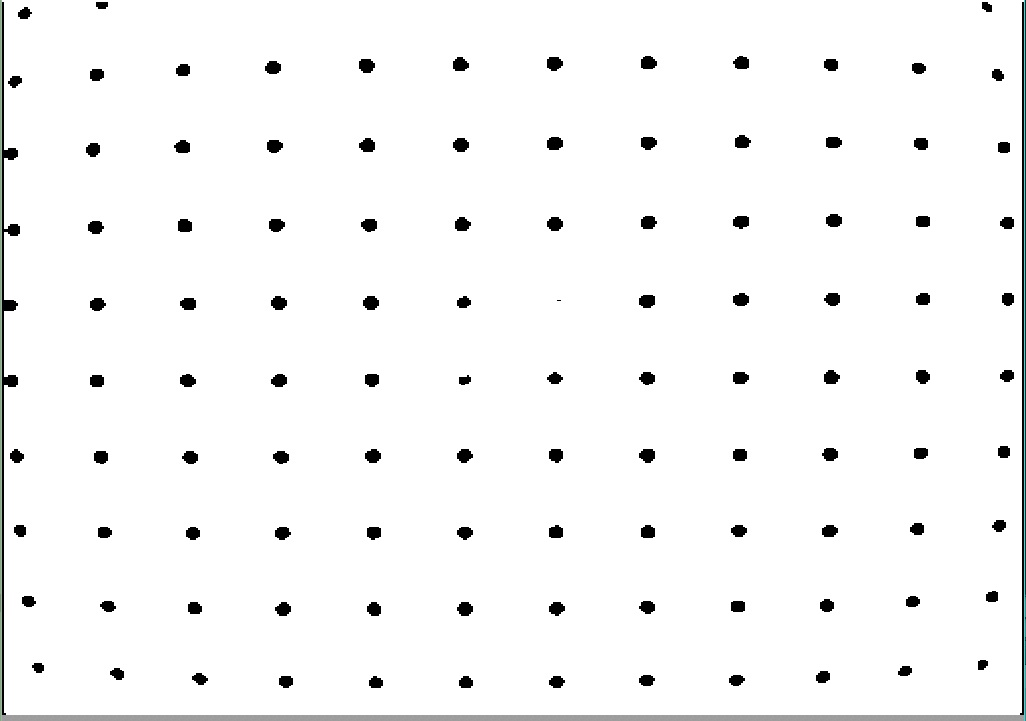
\includegraphics[width=0.5\textwidth]{Binarized_Single_NIR}
\label{Binarized_Single_NIR}}
%\qquad
\subfloat[Dot Centers Extraction][Extracted and Marked]{
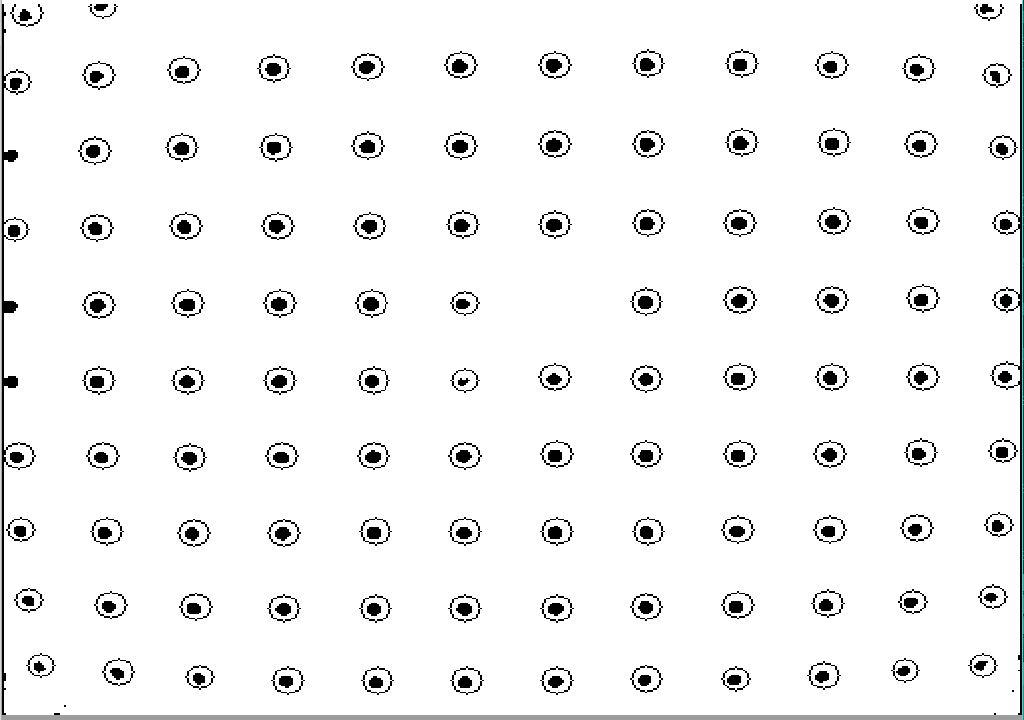
\includegraphics[width = 0.5\textwidth]{Dots_Extracted_Single_NIR}
\label{Dots_Extracted_Single_NIR}}
%
\caption{Valid Dot-Clusters Extracted in \gls{NearIR}}
\label{DotCentersExtraction}
\end{figure}
%%%
%%
%%
\subsection{\((\gls{worldX}, \,\gls{worldY})\) Fitting based on Uniform Grid}
\label{uniformGridFittingXY}
%%
With a list of image space points (\(R, C\))s extracted, the following is to assign those points with their corresponding world coordinates \((\gls{worldX}, \,\gls{worldY})\)s, so that we can get coordinate-pairs to train a mapping model for dense \(X^WY^W\) generation. The world coordinates are based on the uniform grid. Taking the side of unit-square (distance between two adjacent dots) as \enquote{Unit One} in the world coordinates and one dot as the origin of plan \(X^WY^W\), all fitted \(\gls{worldX}\)/\(\gls{worldY}\) values will be integers. %
\\\indent%
Ideally, a $3\times3$ perspective transformation matrix could help set a linear mapping between two different 2D coordinates, and 3 dot centers with known coordinates pair of \((R, C)\) and \((\gls{worldX}, \,\gls{worldY})\) are enough to determine the transformation matrix. Once four points with a squared-shape \(R\)/\(C\) distribution is found, a $3\times3$ perspective transformation matrix \(A\) could be determined by solving 
\begin{equation}
%
\left[ \begin{array}{c} %
zX^W \\ zY^W \\ z \end{array} \right] %
= %
A \left[ \begin{array}{c} %
C \\ R \\ 1 \end{array} \right] %
= %
\begin{bmatrix} 
a_{11} & a_{12} & a_{13} \\
a_{21} & a_{22} & a_{23} \\
a_{31} & a_{32} & a_{33} \\
\end{bmatrix}%
 \left[ \begin{array}{c} %
C \\ R \\ 1 \end{array} \right] %
 \ ,%
\label{perspectiveDistortionCorrectionEquation}
\end{equation}%
%
\noindent
where \(C\) and \(R\) are vectors consist of four squared-shape distributed points' addresses; \(\gls{worldX}\) and \(\gls{worldY}\) are vectors consist of four points \((0, 0)\), \((0, 1)\), \((1, 1)\), and \((1, 0)\); \(z\) denotes the third axis in the homogenous system connecting two coordinates. %
\\\indent%
Deformed by lens distortions, the cluster centers in image plane are not uniformly distributed, and this $3\times3$ transformation matrix can only generate corresponding decimal \(\gls{worldX}\)/\(\gls{worldY}\) values that are close integers. But in practice, the correct integer values \(\gls{worldX}\)/\(\gls{worldY}\) could still be located through \(Rounding\). Considering that a list of cluster centers' image coordinate \((R, C)\)s will give many groups of four squared-shape distributed points, and each of them gives a different image coordinate distance will be mapped to the \enquote{Unit One} in world coordinates, we will traverse all of the possible groups of four squared-shape distributed points and pick out the group whose mapping matrix \(A\) generates the most points that are close to integers. %
%
In this way, we find the transformation matrix \(A\) can give the best \enquote{Unit One} distance in world coordinates. However, its generated point \(\gls{worldX}/\gls{worldY} = 0\) is usually not at the dot-cluster that is closest to the center of cameras' \gls{FoV}. A translation matrix \(T\) could be used to refine the transformation matrix \(A\) and help to translate the origin point to be at the dot cluster we want:%
%
\begin{equation}
%
A_{\text{\_refined}}%
= %
T \cdot A %
= %
\begin{bmatrix} 
1 & 0 & -X_{\text{\_Zero\_A}} \\%
0 & 1 & -Y_{\text{\_Zero\_A}} \\%
0 & 0 &   1 \\%
\end{bmatrix}%
\cdot A%
\, \, \, \ \ ,%
\end{equation}%
%
where \((X_{\text{\_Zero\_A}}, \, Y_{\text{\_Zero\_A}})\) is the integer world space address rounded after the transformation from image space center point:%
%
\begin{equation}
%
\left[ \begin{array}{c} %
zX_{\text{\_Zero\_A}} \\ zY_{\text{\_Zero\_A}} \\ z \end{array} \right] %
= %
A\cdot \left[ \begin{array}{c} %
C_{\text{\_center}} \\ R_{\text{\_center}} \\ 1 \end{array} \right] %
 \ .%
\end{equation}%
\noindent
where \((C_{\text{\_center}}, \, R_{\text{\_center}})\) denotes the center point of \gls{FoV} in image space. Eventually, the refined transformation matrix $A_{\text{\_refined}}$ can help assign world coordinates to the extracted image space coordinates, with the point \(\gls{worldX}/\gls{worldY}=0\) at the dot-cluster nearest to the image center, as shown in Fig.~\ref{XY_GridFitting_Matlab}.
%
 \begin{figure}[t]
\hspace*{-0.3cm}
\centering
\subfloat[Image Plane Coordinates][ImagePlane Coordinate]{
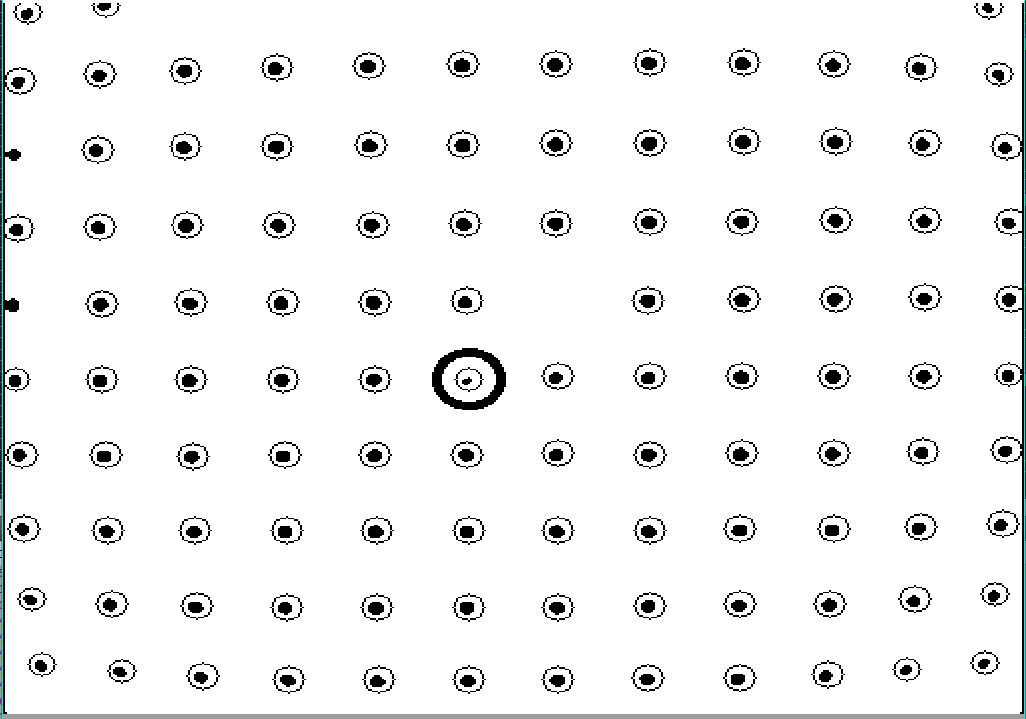
\includegraphics[width=0.54\textwidth, height = 0.425\textwidth]{Grid_Centered_Single_NIR}
\label{Grid_Centered_Single_NIR}}
%\qquad
\subfloat[World Coordinates][World Coordinate]{
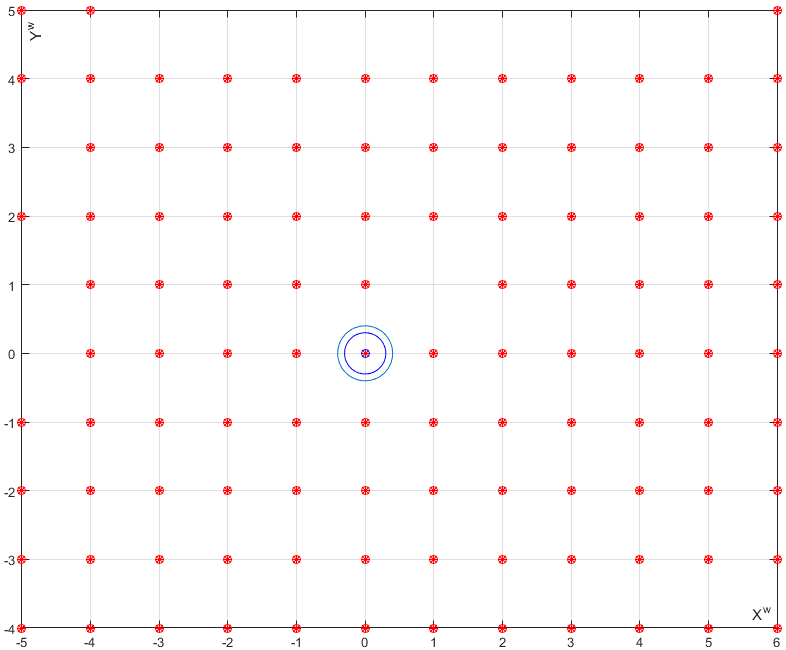
\includegraphics[width = 0.47\textwidth, height = 0.425\textwidth]{XY_GridFitting_Matlab}
\label{XY_GridFitting_Matlab}}
%
\caption{Coordinates-Pairs: (\(R, C\))s and (\(\gls{worldX}\), \(\gls{worldY}\))s}
\label{Grid_Fitting}
\end{figure}%

%%
\subsection{Dense \(\gls{worldX}/\gls{worldY}\) Generation}
\indent
%With a list of points with image space addresses (\(R, C\))s extracted,   
The generation of undistorted dense \(X^WY^W\) needs to consider lens distortion removal. In the traditional calibration method, world space \(\gls{worldX}/\gls{worldY}/\gls{worldZ}\) are mapped to undistorted (\(R', C'\)) by linear pinhole camera matrix \(M\). And then the undistortion step from undistorted (\(R', C'\)) to distorted (\(R, C\)) is done by eqn.~(\ref{lensDistortion}), which uses a high order (higher than 2nd order) polynomial equation. Assuming that there is a high order mapping relationship directly from the distorted image space (\(R, C\)) to world space (\(\gls{worldX}, \, \gls{worldY}\)), we will do different orders of two-dimensional polynomial prototypes in Matlab using its application of \enquote{Curve Fitting Toolbox}, and then decide a best-fit mapping model with a high accuracy and a relative small number of parameters.
%
\\\indent
A two-dimensional polynomial model means surface mapping between two different spaces. Equation.~(\ref{perspectiveDistortionCorrectionEquation}) (perspective correction) as \(1^{st}\) order polynomial mapping is not able to handle lens distortions. 
%
The second order polynomial mapping has $2\times6=12$ parameters, written as %
%
\begin{equation}
\begin{aligned}
\gls{worldX} &=  a_{11}C^2 + a_{12}CR + a_{13}R^2 + a_{14}C + a_{15}R + a_{16}
\\%
\gls{worldY} &=  a_{21}C^2 + a_{22}CR + a_{23}R^2 + a_{24}C + a_{25}R + a_{26} \, , 
\end{aligned}
\label{secondOrderPolynomial}
\end{equation}%
%
\noindent
and similarly, the fourth order polynomial mapping has $2\times15=30$ parameters, given by 
%
\begin{equation}
\hspace*{-0.3cm}%
\begin{aligned}
\gls{worldX} &=  a_{11}C^4 + a_{12}C^3R + a_{13}C^2R^2 + a_{14}CR^3 + a_{15}R^4 + a_{16}C^3 + a_{17}C^2R \ \ \ ...\\%
&\,\,\,\,\,\,+ a_{18}CR^2 + a_{19}R^3 + a_{110}C^2 + a_{111}CR + a_{112}R^2 + a_{113}C + a_{114}R + a_{115}
\\\\%
\gls{worldY} &=  a_{21}C^4 + a_{22}C^3R + a_{23}C^2R^2 + a_{24}CR^3 + a_{25}R^4 + a_{26}C^3 + a_{27}C^2R \ \ \ ...\\%
&\,\,\,\,\,\,+ a_{28}CR^2 + a_{29}R^3 + a_{210}C^2 + a_{211}CR + a_{212}R^2 + a_{213}C + a_{214}R + a_{215}      \,\,.
\end{aligned}
\label{fourthOrderPolynomial}
\end{equation}%
%
\indent
To prototype equation \ref{secondOrderPolynomial} and \ref{fourthOrderPolynomial} in Matlab, \enquote{Curve Fitting Toolbox} is used to obtain the $2\times6$ and $2\times15$ parameters, using 107 points' coordinates pairs of image space \(R/C\) and world coordinates \(\gls{worldX}/\gls{worldY}\). Based on the \enquote{Goodness of fit} of transformation parameters from Matlab, the Root-Mean-Square Error (RMSE) of (\(\gls{worldX}\), \(\gls{worldY}\)) is (0.06796, 0.05638) for the \(2^{nd}\) order polynomial, and (0.02854, 0.02343) for the \(4^{th}\) order polynomial. As the order of polynomial goes higher, the RMSE gets smaller, and the cost of parameters' calculation gets much higher as well. After the prototyping in Matlab, the different orders of polynomial models will be applied into real-time streams transformation to get live transformed world space reconstruction. Eventually, the \(4^{th}\) order polynomial transformation model is selected as the distortion removal mapping model, which can give an intuitive undistorted world space image while costing relative less calculations. This mapping model will be trained by coordinate-pairs of the extracted points, and then be applied to image space addresses to generate dense \(\gls{worldX}/\gls{worldY}\) for all pixels.
%% mapping model parameters determination
%
%
\section{Data Process and \gls{LUT} Generation}
Till now, we have collected frames of \(X^WY^WZ^WRGBD\) data from RGB streams and \(X^WY^WZ^WID\) from \gls{NearIR} stream. The \(X^WY^WZ^WRGBD\) data from RGB streams can be used for color values' alignment after the \gls{3D} reconstruction based on depth stream. Since the \gls{NearIR} stream has same pixel distribution with depth stream, we will process the \(X^WY^WZ^WID\) data and generate per-pixel mapping parameters, which can be saved as \gls{LUT} for undistorted \gls{3D} reconstruction. From section \ref{sectionRailCalibrationSystem}, we know that our whole idea of a calibrated natural \gls{3D} reconstruction on \gls{GPU} is to make use of per-pixel eqn.~(\ref{kaiBeamEquationCh3}), which requires undistorted \(X^WY^WZ^W\) data and a per-pixel mapping from \(\gls{D}\) to \(\gls{worldZ}\). With enough \(X^WY^WZ^WID\) data already been collected, we will determine a per-pixel \(\gls{D}\) to \(\gls{worldZ}\) mapping, and then generate \gls{LUT} for calibrated \gls{3D} reconstruction.
\\\indent
\begin{figure}[b]
\centering
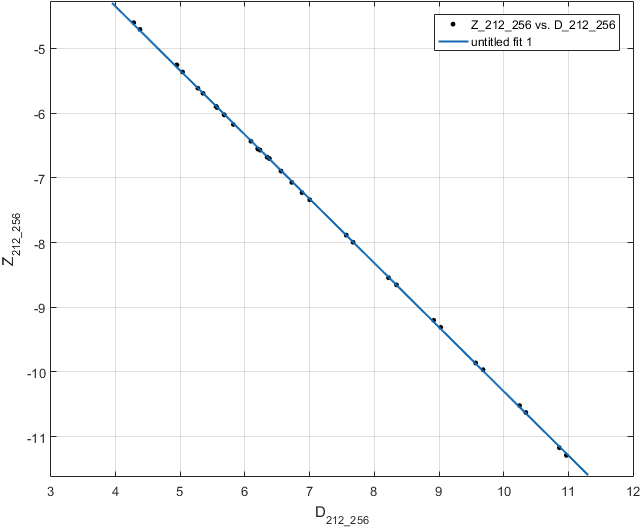
\includegraphics[width=0.55\textwidth]{ZD_CurveFitting}
\caption{Polynomial Fitting between \gls{D} and \(\gls{worldZ}\)}
\label{ZD_CurveFitting}
\end{figure}%
%
Both of \(\gls{D}\) and \(\gls{worldZ}\) are continuous data, so that their function could written as a polynomial expression, based on Taylor series. We will determine a best-fit mapping model from \(\gls{D}\) to \(\gls{worldZ}\) using Matlab. Figure~\ref{ZD_CurveFitting} shows the polynomial fitting result in Matlab \enquote{Curve Fitting Tool} toolbox, with 32 points of \(DZ^\text{W}\) values (at pixel \(\gls{imageColumn}\)=256 and \(\gls{imageRow}\)=212) from 32 frames. It is apparent that \(\gls{worldZ}\) is linear with \(\gls{D}\). Therefore, for every single pixel, \(\gls{worldZ}\) could be mapped from \(\gls{D}\) through \par
%
\begin{equation}
\gls{worldZ}[m, \, n] = e[m, n]\gls{D}[m, \, n]+f[m, n] ,
\label{fromD_To_Z}
\end{equation}%
%
\noindent
where \([m, \, n]\) denotes the image address \(\gls{imageRow}\) and \(\gls{imageColumn}\) of a pixel, \(e/f\) are the corresponding linear coefficients that help map from \(\gls{D}\) to \(\gls{worldZ}\). With eqn.~(\ref{fromD_To_Z}) supporting the per-pixel \(\gls{worldZ}\) values and eqn.~(\ref{kaiBeamEquationCh3}) help generating the per-pixel \(X^WY^W\) values, we found all of the six per-pixel parameters \((a/b/c/d/e/f)\) we need. We are now ready to process the collected data off-line and generate a \(numDepthRows\) by \(numDepthCols\) by 6 \gls{LUT}.
\\\indent
%
 \begin{figure}[t]
\hspace*{-0.5cm}
\centering
\subfloat[Staggered]{
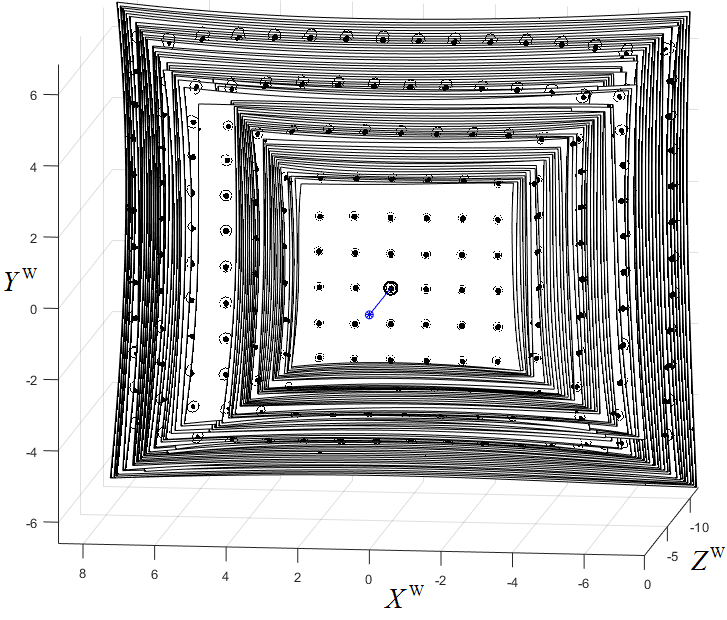
\includegraphics[width=0.5\textwidth]{staggeredPiles}
\label{staggeredPiles}}
%\qquad
\subfloat[Unified]{
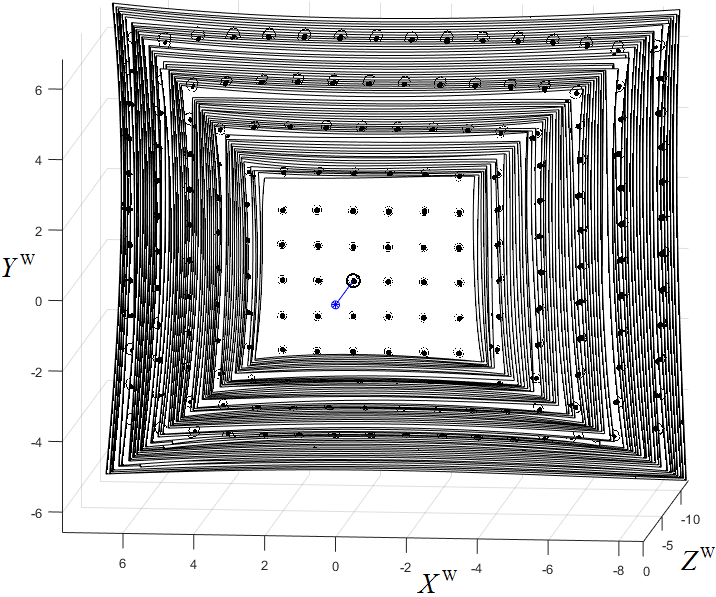
\includegraphics[width = 0.5\textwidth]{unifiedPiles}
\label{unifiedPiles}}
%
\caption{World Space Unification of Collected Data}
\label{worldSpaceDataUnification}
\end{figure}
%
The collected data cannot be used directly for \gls{LUT} generation, because \(\gls{worldX}/\gls{worldY}\) may not be well aligned and pre-processes of data are needed. Our calibration system did not require the camera's observing orientation to be along with \(\gls{worldZ}\)-axis, which results to the fact that, the collected frames might be staggered when the centered dot-cluster in camera's \gls{FoV} moves. Figure~\ref{staggeredPiles} shows the raw collected data before world space unification, which has a staggered piles of frames. In order to make the data available for generating valid per-pixel \gls{3D} reconstruction parameters, we need to unify their world space by adding or subtracting a corresponding integer to all pixels in every staggered frame, making sure the point \(X^WY^W = 0\) is at the same dot-cluster for all frames.	After the data unification of world space, as shown in Fig.~\ref{unifiedPiles}, we are all ready to determine the per-pixel mapping parameters \(a/b/c/d/e/f\) and generate the \gls{LUT}.
%\subsection{Mathematical tools}
%\subsubsection{Singular Value Decomposition (SVD)}
%\subsubsection{Least Square with Pseudo-Inverse}
%
\section{Alignment of RGB Pixel to Depth Pixel}
Now an undistorted \gls{3D} reconstruction could be displayed with the help of the calibrated \gls{LUT}. However, we have not figured out yet what the color of each pixel is. To generate a colored \gls{3D} reconstruction with a combination of a random depth sensor and a random RGB sensor, we need to align the RGB pixels to depth pixels. The intermediate between the depth sensor image space and RGB sensor image space is the world space. As long as we figure out the mapping from world space to RGB sensor image space, the color of pixel with known \(X^WY^WZ^W\) could be looked up from the RGB image space. The pinhole camera matrix \(M\) is used to map from world space to RGB image space. Using the frame data from Kinect RGB steams and Kinect \gls{NearIR} streams, a Matlab prototype of RGB pixels alignment is shown in Fig.~\ref{RGBAligned_Matlab}, where the RGB textured is mapped onto its corresponding \gls{NearIR} image, who has same pixels with depth sensor. The total black area on the top edge and bottom edge is where the depth sensor's view goes beyond the RGB sensor's view. Figure~\ref{RGBvaluesAligmentMatlabQt} shows the screen-shot of live video after calibration with the RGB pixels aligned by a pinhole camera model \(M\).

%
 \begin{figure}[h]
\hspace*{-0.5cm}
\centering
\subfloat[][]{
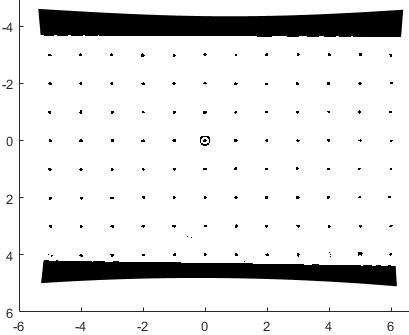
\includegraphics[width = 0.5\textwidth]{RGBAligned_Matlab}
\label{RGBAligned_Matlab}}
\subfloat[][]{
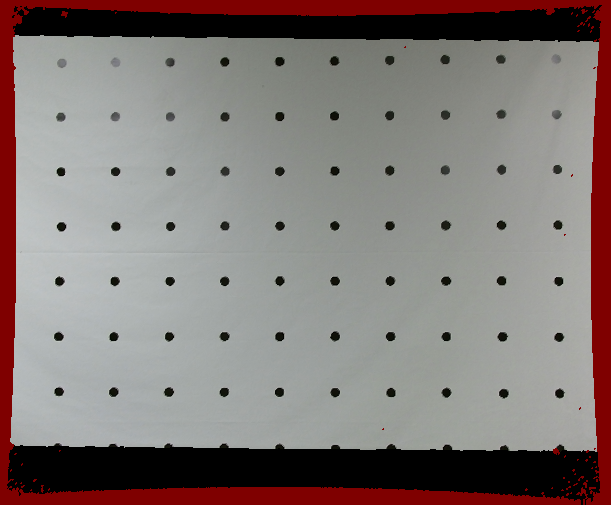
\includegraphics[width=0.5\textwidth]{RGBAligned_Qt}
\label{RGBAligned_Qt}}
\caption{Alignment of RGB Texture onto \gls{NearIR} Image}
\label{RGBvaluesAligmentMatlabQt}
\end{figure}%
%

%	
%%	
%\section{Summation}
%A per-pixel calibration method, using a moving plane calibration system, is proposed in this chapter. The main idea of this calibration method is to make it available to generate accurate (undistorted) per-pixel world space position (\(\gls{worldX}, \, \gls{worldY}, \, \gls{worldZ}\)) directly in real-time with the fewest calculation. The per-pixel \(\gls{worldZ}\) will be mapped from per-pixel depth value \(\gls{D}\), and then per-pixel \(\gls{worldX}/\gls{worldY}\) will be determined by per-pixel linear beam equation from its corresponding \(\gls{worldZ}\). Note that the per-pixel beam equation represents the lens-distortion removed field of view of a single pixel. And the \enquote{depth distortion} could be removed during the per-pixel mapping from \(\gls{D}\) to \(\gls{worldZ}\). In short, this per-pixel calibration method consists of two big steps: \(X^WY^WZ^W+\gls{D}\) data collection and mapping parameters determination. \(\gls{D}\) is simply from depth streams. \(\gls{worldZ}\) is from external based on the camera's position on the rail. And the undistorted (\(\gls{worldX}, \, \gls{worldY}\)) are from the transformation of \(R/C\) by a \(4^{th}\) order polynomial mapping model, during which lens-distortions could be removed. With the frames data of \(X^WY^WZ^W+\gls{D}\) collected, the per-pixel mapping parameters \(a/b/c/d/e/f\) could be determined by eqn.~(\ref{fromD_To_Z}) and eqn.~(\ref{kaiBeamEquationCh3}). 
%\\\indent
%Without using the traditional pinhole camera model, two polynomial mapping models are employed in this calibration method. The first model is the two-dimensional \(4^{th}\) order polynomial mapping from \(R/C\) to \(\gls{worldX}/\gls{worldY}\) during the frames data collection, which takes care of the removal of lens distortions; and the second model is the linear mapping from \(\gls{D}\) to \(\gls{worldZ}\), which can handle \enquote{depth distortion}. Both of the two mapping models are determined and calculated by real streams data from the camera, so that we claim this per-pixel calibration method a \enquote{data-based} calibration method. 
%\\\indent
%Besides the data-based calibration method, a robust \gls{DIP} process during calibration is also discussed, which guarantees that the live video during undistorted frames collection could be in real-time. Note that \enquote{real-time} here means being able to show an undistorted frame before the start of the second frame processing. After the undistorted \gls{3D} reconstruction, the alignment of the RGB pixel to Depth pixel is also discussed. The data-based calibration method could be applied universally on any \gls{RGBD} cameras. With the alignment of RGB pixels, it could even work on the combined \gls{3D} camera of a random Depth sensor and a random RGB sensor.

















%
%
% Kai \cite{Kai10} shows that, \gls{GPU} programing is ideally suited to this kind of per-pixel processing. He did a good job on structed light \gls{3D} scanner parallel calibration on \gls{GPU}, and derived the per-pixel beam equation~(\ref{kaiBeamEquationCh3}) directly from a pinhole camera matrix \(M\). 
%%
%\begin{equation}
%\begin{aligned}
%\gls{worldX}[m,\,  n] = c[m, n]\gls{worldZ}[m,\,  n]+d[m, n]
%\\%
%\gls{worldY}[m,\,  n] = e[m, n]\gls{worldZ}[m,\,  n]+f[m, n]
%\end{aligned}
%\label{kaiBeamEquationCh3}
%\end{equation}%
%\noindent
%where [\(m,n\)] is the discrete space \(\gls{imageRow}\) and \(\gls{imageColumn}\) coordinate of each pixel in a M by N sensor. This per-pixel beam equation shows per-pixel linear mappings from \(\gls{worldZ}\) to \(\gls{worldX}/\gls{worldY}\), and the per-pixel \(\gls{worldZ}\) can be mapped from features of structured light. 
%\\\indent
%Without calibration, we can also derive per-pixel beam equations in camera space and apply them in \gls{GPU} parallel processing. In this section, we will introduce how to draw a colored camera space \gls{3D} reconstruction on \gls{GPU} without calibration, using a \gls{KinectV2} camera. As shown in the diagram in Fig.~\ref{cameraSpaceDiagram}, we will retrieve \(Depth\), \(RGB\) and \(mapping\) streams from the \gls{KinectV2} camera, and save them into corresponding buffers respectively. The mapping streams contains \(\gls{imageRow}\) and \(\gls{imageColumn}\) values that can help every depth pixel to look for color infos from \(RGB\) streams. Then those three streams will be uploaded from CPU onto \gls{GPU} as textures for image drawing. The camera space \gls{3D} coordinates \(X^CY^CZ^C\) for the final \gls{3D} image will be generated based on depth texture, which will also be processed on \gls{GPU} in the way that similar to drawing colors on a pixel. In short, we will draw on \gls{GPU} twice: one for camera space coordinates generation and \(RGB\) alignment, the other one for real \gls{3D} image drawing.
%\\\indent
%
%In the first drawing step of camera space coordinates generation, a look-up texture will be created for the final \gls{3D} image drawing, which contains both camera space coordinates and color (RGB) values. To draw a certain color on one single pixel, \gls{GPU} provide one single fragment shader to generate and save corresponding four color channel RGBA (A for alpha, opacity) single-floating data into a corresponding position in a framebuffer. We could take the framebuffer as a screen on which we are going to draw, and the positions in the framebuffer would be same with pixels in the screen. We will follow the way how \gls{GPU} do drawing, and use \gls{GPU} to calculate per-pixel \(X^CY^CZ^C\) and save the calculation results with RGB streams together as total six channels into a customer framebuffer. The first thing is to initial a customer framebuffer, whose texture will finally be utilized to look up per-pixel's \(X^CY^CZ^CRGB\) six channels of data for the eventual \gls{3D} image drawing. The internal texture format of {\ttfamily\color[rgb]{0.0,0.0,0.5019608}GL\_RGBA32F}, which means one pixel position (\(\gls{imageRow}\), \(column_0\)) can contain four channels. We need a second position (\(\gls{imageRow}\), \(column_0 + 1\)) for every single pixel to contain the total six channels. Therefore the customer framebuffer will be initialed with a size of %
%({\ttfamily
%\textcolor[rgb]{0.0,0.0,0.5019608}{2}\textcolor{black}{* }\textcolor[rgb]{0.5019608,0.0,0.0}{numDepthCols}\textcolor{black}{, }\textcolor[rgb]{0.7529412,0.7529412,0.7529412}{
% }\textcolor[rgb]{0.5019608,0.0,0.0}{numDepthRows}}),
%where numDepthRows and numDepthCols denote the size of total rows and total columns of the depth sensor. %
%\\\indent
%Four corner points coordinates, as four vertices, will be uploaded onto vertex shader to form a quadrilateral filling up the screen, which will cover the numDepthRows by (2*numDepthCols) framebuffer. With respect to a random position of every single depth pixel, two corresponding \enquote{virtual pixels} (positions) will be processed by two independent fragment shaders to respectively save \(X^CY^CZ^C\) and \(RGB\) data into the customer framebuffer. The fragment shader is programmed as below.
%\\%
%%
%This fragment shader handles both of \(X^CY^CZ^C\) generation and \(RGB\) texel fetch. There are four uniform input textures uploaded on \gls{GPU}. The \emph{qt\_colorTexture} is RGB stream, and \emph{qt\_depthTexture} is depth stream. \emph{qt\_mappingTexture} is a mapping stream also given by \gls{KinectV2} camera, which contains two channels \(Row/Col\) mapping data. It offers a link between RGB stream and Depth stream, helping align RGB values to depth pixels. \emph{qt\_spherTexture} is a per-pixel beam mapping texture created by ourselves, which helps map from \(\gls{cameraZ}\) to \(\gls{cameraX}/\gls{cameraY}\) respectively based on the horizontal and vertical field of view of a pinhole camera model. Let's view the fragment shader step by step, and then talk about the creation of beam mapping texture in detail.%
%\\\\
%We will first get the texture coordinates from the fragment coordinates.
%\\\\
%    ivec2 textureCoordinate = ivec2(gl\_FragCoord.x/2, gl\_FragCoord.y);
%\\\\
%And then have a check if this fragment shader should be assigned for \(X^CY^CZ^C\) generation, or \(RGB\) texel fetch.\\\\
%    if (int(gl\_FragCoord.x)\%2 == 0)\{\\
% 		// \(X^CY^CZ^C\) generation
%    \} else \{
%		// \(RGB\) texel fetch
%    \}%
%%
%\\\\
%The depth steam measures \(\gls{cameraZ}\), which after rescaling is given by :
%\\\\
%        float z = texelFetch(qt\_depthTexture, ivec2(col, textureCoordinate.y), 0)[chn] * 65130.0 - 20.0;
%\\\\
%
%Based on the pinhole-camera model, we could derive a per-pixel proportional mapping from \(\gls{cameraZ}\) to \(\gls{cameraX}/\gls{cameraY}\) using the horizontal and vertical Field of View. In a depth sensor of size %
%({\ttfamily
%\textcolor[rgb]{0.5019608,0.0,0.0}{numDepthCols}\textcolor{black}{, }\textcolor[rgb]{0.7529412,0.7529412,0.7529412}{
% }\textcolor[rgb]{0.5019608,0.0,0.0}{numDepthRows}}),
%%
%a pixel with image address (\(Row, \, Col\)) has its view in camera space as a beam passing through the camera space origin (the pin hole). For one specific camera with a certain filed of view, a pixel's beam function depends on its address (\(Row, \, Col\)). As shown in Fig.~\ref{VHfieldOfView}, the relationship between a pixel's beam view (\(\gls{cameraZ}\) to \(X^CY^C\)) and the sensor's vertical / horizontal Field of View could be expressed as eqn.~(\ref{pinholeProportionZXY}).
%%
%\begin{equation}
%\begin{aligned}
%\frac{\gls{cameraX}_{[Row, \, Col]}}{\gls{cameraZ}_{[Row, \, Col]} \times tan(horFoV / 2)} 
%=
%%tan\bigg[
%%	Hor\text{\gls{FoV}}
%%		\bigg(
%			\frac{Col}{numDepthCols} - 0.5
%%		\bigg)
%%\bigg]
%\\\\%
%\frac{\gls{cameraY}_{[Row, \, Col]}}{\gls{cameraZ}_{[Row, \, Col]} \times tan(verFoV / 2)} 
%=
%%tan\bigg[
%%	Ver\text{\gls{FoV}}
%%		\bigg(
%			\frac{Row}{numDepthRows} - 0.5
%%		\bigg)
%%\bigg]
%\end{aligned}
%\label{pinholeProportionZXY}
%\end{equation}%
%
%\noindent
%From eqn.~\ref{pinholeProportionZXY}, we could generate a per-pixel beam mapping texture which contains the proportion parameters that can map from per-pixel \(\gls{cameraZ}\) to per-pixel \(\gls{cameraX}/\gls{cameraY}\).
%\\\\
%        vec4  a = texelFetch(qt\_spherTexture, textureCoordinate, 0);\\
%        // CONVERT SPHERICAL COORDINATES TO CARTESIAN\\
%        qt\_fragColor.x = -z * a.r;\\
%        qt\_fragColor.y = -z * a.g;\\\\































































%In our calibration system, 



%
%%%
%%%
%%%
%\indent From Chapter \ref{chapterTraditionalCalibration} we know one dimension calibration method is suitable for calibrating multiple cameras together; three dimension object calibration has the highest accuracy but also cost more on system setup; two dimension plane calibration owns both of good accuracy and simple setup. However, those traditional calibration methods are not ideal enough while considering that researchers are chasing after accuracy. Either that, the static calibration pattern does not have enough points to offer distortions' information. Concretely only few limited points could be extracted in the three dimension calibration system as shown in Fig.~\ref{threeDSixPointsCalibrating}. Or, it is hard to control the extracted calibration points to cover enough area of the image space in the famous two dimension calibration methods. Fig.~\ref{simulatedMultiPlanesCheckerboard} shows the simulated multiple planes of checkerboard with respect to the camera space, with data from the two dimension calibration method that is employed in both of Matlab and OpenCV applications, to intuitively inspect the extrinsic parameters. Using this method, researchers need to manually keep changing their poses of holding the checkerboard, in order to get enough calibration points to cover all of the image space area. Besides, all of the traditional calibration methods are assuming that the depth sensor offers perfect accurate \(\gls{cameraZ}\) values for all of its pixels, \textit{i.e.}, \(\gls{cameraZ}_{[row, col]} - Depth_{[row, col]} = E_{\text{Constant}}\) such that for all image space range of \([row,\, col]\) pixels  share one same error \(E_{\text{Constant}}\). But in practice, depth sensors always have some defects in getting same depth accuracy for all of their pixels, which we will call as \enquote{Depth Distortion}. As shown in Fig.~\ref{NIR_by_Depth_LeftSide}, even observing a flat wall there are still many bumps and hollows in the reconstructed \gls{3D} image.
%%
% \begin{figure}[b]
%%\hspace*{-0.5cm}
%\centering
%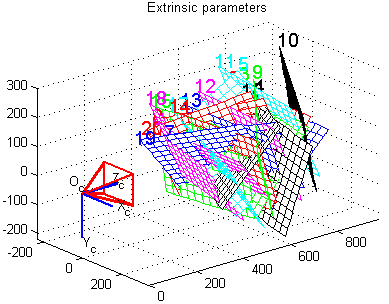
\includegraphics[width=0.55\textwidth]{simulatedMultiPlanesCheckerboard}
%\caption{Simulated Planes of Checkerboards showing Extrinsic Parameters}
%\label{simulatedMultiPlanesCheckerboard}
%\end{figure}%
%%
%%
%\\\indent
%Most of those defects in the methods discussed above are based on the losing control of the calibration points. Even though a flexible two dimension calibration method got its camera observing orientations easily changed by hand, it is almost impossible to numerically locate all desired poses that can make calibration points fill up all image space area. However, Tsai's old calibration system, which requires a known motion of the plane, can make them up. It has been obsoleted nowadays due to the fact that knowing the motion is not necessary for determining the intrinsic and extrinsic parameters. But as the resolution of camera sensor gets higher and higher, like a high definition sensor, researchers need a better calibration system. What's more, with the motion of the calibration plane controllable, it will not be a problem to determine the mapping from \(Depth (\gls{D})\) to \(\gls{worldZ}\), thus equation \ref{kaiBeamEquation} could be applied as one important step to simplify \gls{3D} reconstruction using a look-up table (lut) after calibration. Note that, both of the mapping from \(\gls{D}\) to \(\gls{worldZ}\) and the coefficients \(c/d/e/f\) help map from \(\gls{worldZ}\) to \(\gls{worldX}/\gls{worldY}\) are with respect to per-pixel, such that even the \enquote{Depth Distortion} could be calibrated.
%
%\section{Novel Per-Pixel Calibration Method}
%\label{sectionPerPixelCalibration}
%In this thesis, we build a moving plane calibration system collecting tree dimensional data, with a rail that gets the \gls{RGBD} camera mounted on its slider observing a planar pattern. The \gls{3D} camera we used is \gls{KinectV2}, but the calibration method could be applied on any \gls{RGBD} cameras. As shown in Fig.~\ref{trackingModuleOnKinectV2CalibrationSystem}, a uniform grid dots pattern is hung on the wall, and the rail is perpendicular to the wall. We will assign the wall, on which the canvas is hung and printed with uniform grid dots pattern, as the \(X^WY^W\) plane in world space, and \(\gls{worldZ}\)-axis would be along the rail. The \gls{RGBD} camera waiting to calibrate is mounted on the slider. Note that, in this calibration system, the only unit that needs to be perpendicular to the wall is the rail, whereas the \gls{RGBD} camera has no need to require its observation orientation. Because all of the mappings we are going to determine are with respect to per-pixel, \textit{i.e.}, the calculated parameters group for every single pixel, which will determine the pixel's view, are independent with that of the other pixels. As the slider moves along the rail, the planar dots pattern hung on the wall is moving further with respect to the \gls{RGBD} camera. This rail offers the possibility of taking infinite various frames of various camera working distances (or \(\gls{cameraZ}\)). Although the dots pattern hung on the wall for camera calibration is static itself, however, the dots distributions would be dynamic (covering every single pixel) in the image space when counted together in all of those various frames of various \(\gls{cameraZ}\). 
%\\\indent%
%%how to per-pixel calibrate ?
%In this per-pixel calibration method, we directly focus on the view of every single pixel, the beam. Inspired by Kai (eqn.~\ref{kaiBeamEquation}), our camera calibration method consists of two big steps: frames (\(X^\text{W}Y^\text{W}\gls{worldZ}+\gls{D}\)) data collection, plus per-pixel mapping parameters determination after frames collection; \textit{i.e.}, to collect frames data of \(\gls{worldZ}\) from external and (\(\gls{worldX}, \, \gls{worldY}\)) by a transformation from (\(R, C\)), plus to calculate per-pixel parameters that help map from \(\gls{D}\) to \(\gls{worldZ}\) and \(c/d/e/f\) in eqn.~\ref{kaiBeamEquation} that map from \(\gls{worldZ}\) to \(\gls{worldX}/\gls{worldY}\). Note that, neither have we decided the mapping model from \(\gls{D}\) to \(\gls{worldZ}\), nor from (\(R, C\)) to (\(\gls{worldX}, \, \gls{worldY}\)). We save the flexibilities between accuracy and complexity for now, and will decide those two models based on data.
%\\\indent%
%% World Coordinates assignment
%Assuming the total size of the depth sensor is as small as a point, and the \(\gls{worldZ}\)s for all of the pixels in one frame would share the same value, which could be measured by a laser distance measurer nearby the camera. To simplify the digital image processing (\gls{DIP}) when extracting a desired point (\(R,\, C\)), which will soon be discussed in section \ref{sectionDIPTechniques}, we assign the \enquote{2D origin} (\(\gls{worldX}/\gls{worldY}\) = 0) of world space coordinates at the center of the dot which is closest to the center of the camera's field of view. And the laser measurer spot nearby the camera to at \(\gls{worldZ}\)=0, such that \(Z^{W}\) values are always negative. Note that, the final assigned world space origin (\enquote{\gls{3D} origin}) is not necessarily be where the camera sensor is. It depends on the camera's observation orientation, whose changing leads to the change of the \enquote{2D origin} (and finally change the \gls{3D} origin).
%%%Zw collection
%%%Zw collection
%%%Zw collection
%%%
%\\\\\indent
%In our calibration system, \(Z^{W}\) values for all pixels of every frame will be supported from external laser distance measurer. The \enquote{Unit One} of \(Z^{W}\) value is assigned to be same with the side of unit-square of the uniform grid pattern, which can simplify the \gls{DIP} processing of (\(C, \, R\)) extraction. Concretely, the distance between every two adjacent dots' centers in real-world is 228mm. Therefore, \(Z^{W}\) = -\(Z\)(mm) / 228(mm), where \(Z\) is the distance in reality from the camera to dots-pattern plane along the rail. Fig.~\ref{OneFrameXYZ_Calibrated} shows one sample frame of \gls{3D} reconstruction in the assigned world space, where both of the origin and \(Z\)-axis are high-lighted in blue.
%%
%\begin{figure}[!t]
%\centering
%%calibrated \(X^{W}\)/\(Y^{W}\) and \(Z^{W}\)
%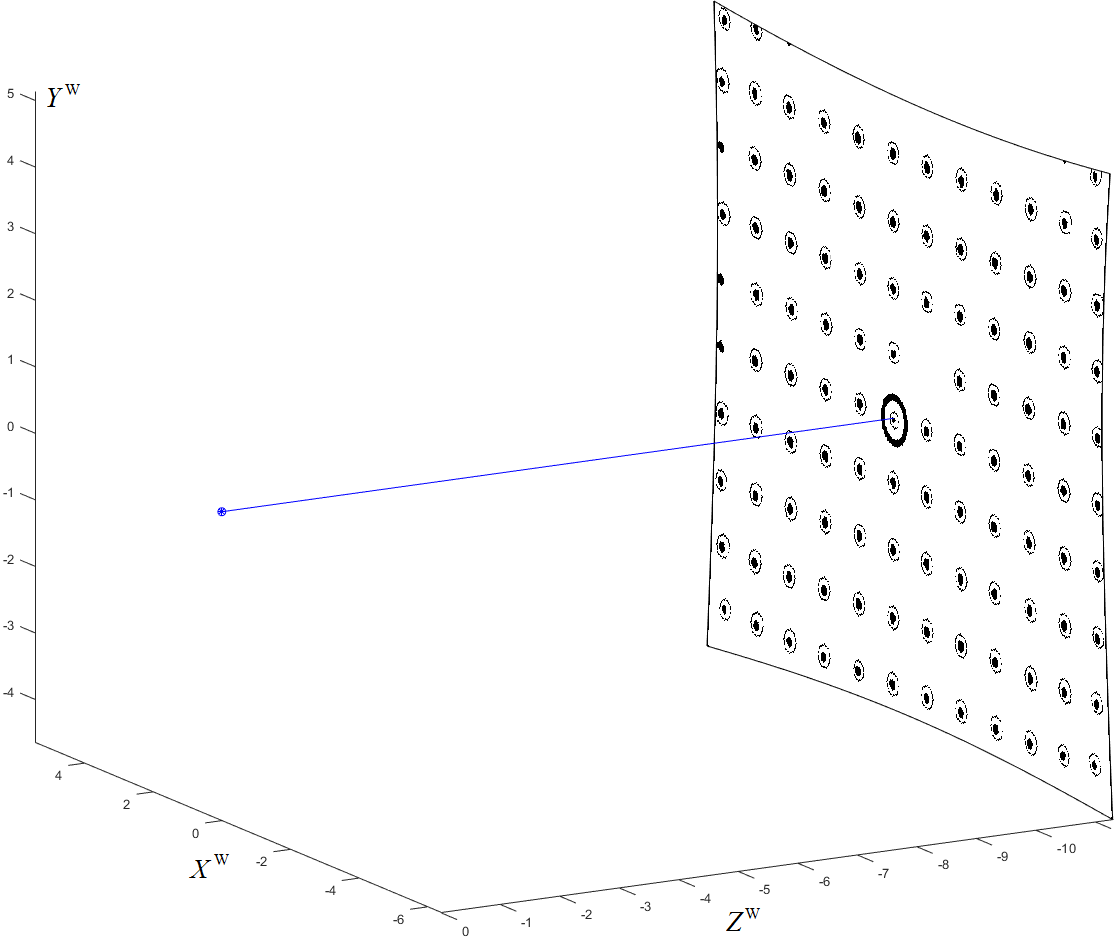
\includegraphics[width=0.7\textwidth, height= 0.5\textwidth]{OneFrameXYZ_Calibrated}
%\caption{\gls{NearIR} \(X^{W}Y^{W}Z^{W}\) \gls{3D} Reconstruction}
%\label{OneFrameXYZ_Calibrated}
%\end{figure}%
%%
%%%
%%%XwYw collection
%%%XwYw collection
%%%XwYw collection
%%%
%\\\indent
%As for (\(\gls{worldX}, \, \gls{worldY}\)) values' collection, a transformation from (\(R, C\)) is needed, during which the lens distortions correction must be considered. In the traditional calibration method, world space \(\gls{worldX}/\gls{worldY}/\gls{worldZ}\) are mapped to undistorted (\(R', C'\)) by linear pinhole camera matrix \(M\). And then the undistortion step from undistorted (\(R', C'\)) to distorted (\(R, C\)) is done by eqn.~\ref{lensDistortion}, which uses a high order (higher than 2nd order) polynomial equation. Assuming that there is a high order mapping relationship directly from the distorted image space (\(R, C\)) to world space (\(\gls{worldX}, \, \gls{worldY}\)), we will do different orders of two-dimensional polynomial prototypes in Matlab using its application of \enquote{Curve Fitting Toolbox}, and then decide a best-fit mapping model with a high accuracy and a relative small number of parameters.
%%
%\\\indent
%A $3\times3$ linear transformation matrix \(A\) (as \(1^{st}\) order polynomial) is usually used for perspective distortion correction, give by eqn.~\ref{perspectiveDistortionCorrectionEquation}. We will try the perspective distortion correction to check if it will also work on the lens distortion correction.
%%
%\begin{equation}
%%
%\left[ \begin{array}{c} %
%zX^W \\ zY^W \\ z \end{array} \right] %
%= %
%A\cdot \left[ \begin{array}{c} %
%C \\ R \\ 1 \end{array} \right] %
%= %
%\begin{bmatrix} 
%a_{11} & a_{12} & a_{13} \\
%a_{21} & a_{22} & a_{23} \\
%a_{31} & a_{32} & a_{33} \\
%\end{bmatrix}%
%\cdot \left[ \begin{array}{c} %
%C \\ R \\ 1 \end{array} \right] %
%%
%\label{perspectiveDistortionCorrectionEquation}
%\end{equation}%
%%
%\noindent
%A two-dimensional polynomial model means surface mapping between two different spaces. The second order polynomial mapping has $2\times6=12$ parameters, written as %
%%
%\begin{equation}
%\begin{aligned}
%\gls{worldX} &=  a_{11}C^2 + a_{12}CR + a_{13}R^2 + a_{14}C + a_{15}R + a_{16}
%\\%
%\gls{worldY} &=  a_{21}C^2 + a_{22}CR + a_{23}R^2 + a_{24}C + a_{25}R + a_{26} \, , 
%\end{aligned}
%\label{secondOrderPolynomial}
%\end{equation}%
%%
%\noindent
%and similarly, the fourth order polynomial mapping has $2 \times 15$=30 parameters, given by eqn.~\ref{fourthOrderPolynomial}.%
%%
%\begin{equation}
%\hspace*{-0.3cm}%
%\begin{aligned}
%\gls{worldX} &=  a_{11}C^4 + a_{12}C^3R + a_{13}C^2R^2 + a_{14}CR^3 + a_{15}R^4 + a_{16}C^3 + a_{17}C^2R \\%
%&\,\,\,\,\,\,+ a_{18}CR^2 + a_{19}R^3 + a_{110}C^2 + a_{111}CR + a_{112}R^2 + a_{113}C + a_{114}R + a_{115}
%\\\\%
%\gls{worldY} &=  a_{21}C^4 + a_{22}C^3R + a_{23}C^2R^2 + a_{24}CR^3 + a_{25}R^4 + a_{26}C^3 + a_{27}C^2R \\%
%&\,\,\,\,\,\,+ a_{28}CR^2 + a_{29}R^3 + a_{210}C^2 + a_{211}CR + a_{212}R^2 + a_{213}C + a_{214}R + a_{215}
%\end{aligned}
%\label{fourthOrderPolynomial}
%\end{equation}%
%%
%\indent
%To prototype equation \ref{secondOrderPolynomial} and \ref{fourthOrderPolynomial} in Matlab, \enquote{Curve Fitting Toolbox} is used to obtain the $2\times6$ and $2\times15$ parameters, using 107 points' coordinates pairs of image space \(R/C\) and world coordinates \(\gls{worldX}/\gls{worldY}\). Based on the \enquote{Goodness of fit} of transformation parameters from Matlab, the Root-Mean-Square Error (RMSE) of (\(\gls{worldX}\), \(\gls{worldY}\)) is (0.06796, 0.05638) for the \(2^{nd}\) order polynomial, and (0.02854, 0.02343) for the \(4^{th}\) order polynomial. As the order of polynomial goes higher, the RMSE gets smaller, and the cost of parameters' calculation gets much higher as well. After the prototyping in Matlab, the different orders of polynomial models will be applied into real-time streams transformation to get live transformed world space reconstruction. Eventually, the \(4^{th}\) order polynomial transformation model is selected as the distortion removal mapping model, which can give an intuitive undistorted world space image while costing relative less calculations. Detailed results and comparisons will be shown soon in section~\ref{sectionPrototypeTwoDtransformation}.
%\\\\\indent
% %% mapping model parameters determination
%%
%\begin{figure}[b]
%\centering
%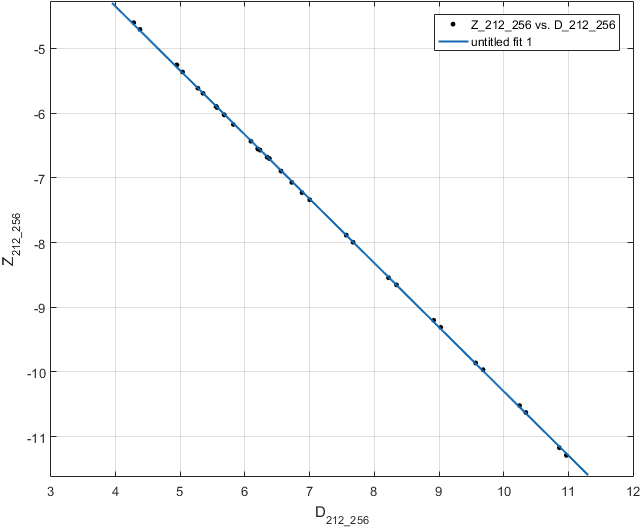
\includegraphics[width=0.55\textwidth]{ZD_CurveFitting}
%\caption{Polynomial Fitting between \gls{D} and Z}
%\label{ZD_CurveFitting}
%\end{figure}%
%%
%Till now, the mapping model from (\(R, C\)) to (\(\gls{worldX}, \, \gls{worldY}\)) has been decided, with which the data collection of \(X^\text{W}Y^\text{W}\gls{worldZ}+\gls{D}\) is ready to be completed. With enough data, the four per-pixel parameters in the beam equation \ref{kaiBeamEquation} are now able to be calculated. In the meanwhile, a best-fit mapping model from \(\gls{D}\) to \(\gls{worldZ}\) could also be determined. Both of \(\gls{D}\) and \(\gls{worldZ}\) are continuous data, so that their function could written as a polynomial expression, based on Taylor series. Fig.~\ref{ZD_CurveFitting} shows the polynomial fitting result in Matlab \enquote{Curve Fitting Tool} toolbox, with 32 points of \(DZ^\text{W}\) values (at pixel \(\gls{imageColumn}\)=256 and \(\gls{imageRow}\)=212) from 32 frames. It is apparent that \(\gls{worldZ}\) is linear with \(\gls{D}\), which is also reasonable. Therefore, for every single pixel, \(\gls{worldZ}\) could be mapped from \(\gls{D}\) through \par
%%
%\begin{equation}
%\gls{worldZ}_{[row, \, col]} = a_{[row, col]}\gls{D}_{[row, \, col]}+b_{[row, col]} ,
%\label{fromD_To_Z}
%\end{equation}%
%%
%\noindent
%where \({[row, \, col]}\) denotes the address of a pixel, \(a/b\) are the corresponding linear coefficients that help map from \(\gls{D}\) to \(\gls{worldZ}\). With eqn.~\ref{fromD_To_Z} supporting the per-pixel \(\gls{worldZ}\) values, eqn.~\ref{kaiBeamEquation} help generating the per-pixel \(X^WY^W\) values, all of the \gls{3D} camera's per-pixel calibration is now done, and we are all ready to show an undistorted \gls{3D} \(X^WY^WZ^W\) reconstruction image.
%%
%%
%%
%%
%\section{\gls{DIP} Techniques on (\(R,\, C\)) Extraction}
%\label{sectionDIPTechniques}
%%  add noises analysis
%\noindent
%In order to train the \(4^{th}\) order mapping model that can map from (\(R, \, C\)) to (\(\gls{worldX}, \, \gls{worldY}\)), we need to obtain at least 15 points' coordinate-pairs of both image space coordinates and world space coordinates. Therefore, a robust \gls{DIP} process to extract the points' addresses (\(R,\, C\))s is of the top priority. Concretely in this project, we are going to extract the dot-clusters' centers from \gls{KinectV2} \gls{NearIR} steams using \gls{DIP} techniques. To guarantee a robust processing, the extraction steps consist of gray-scaling, histogram equalization, adaptive thresholding and a little trick on black pixels counting. OpenGL is selected as the CPU image processing language. The default data type of steams saved on \gls{GPU} during processing is single-floating, with a range from 0 (balck) to 1 (white). 
%\\\indent
%Gray-scaling is done in order to suit for both of the RGB and the \gls{NearIR} steams. For \gls{NearIR} steam, its data contains only color gray. There is no need to consider gray-scale problem, and data will be saved on \gls{GPU} as single-floating automatically. Whereas for RGB steam, a conversion from RGB to gray value is needed. Typically, there are three converting methods: lightness, average, and luminosity. The luminosity method is finally chosen as a human-friendly way for gray-scaling, because it uses a weighted average value to account for human perception, which is give by eqn.~\ref{luminosityGrayScaling}.
%\\\indent
%%
%\begin{equation}
%Intensity_{\text{\_gray}} =  0.21 Red\,  + \, 0.72 Green \, + \, 0.07 Blue
%\label{luminosityGrayScaling}
%\end{equation}%
%%
%As values saved on \gls{GPU}, all of the pixel intensity values are within the range of [0, 1], where \enquote{0} means 100\% black and \enquote{1}  means 100\% white. In practice, \gls{NearIR} steam image is always very dark, as shown in Fig.~\ref{Raw_Single_NIR} (with their intensity values every close to zero).  In order to enhance the contrast of \gls{NearIR} image for a better binarizing, rescaling is necessary. In this section, histogram equalization technique is used maximize the range of valid pixel intensity distributions. Same process is also compatible on the RGB steam.
%%
% \begin{figure}[t]
%\hspace*{-0.5cm}
%\centering
%\subfloat[Raw \gls{NearIR}][Raw]{
%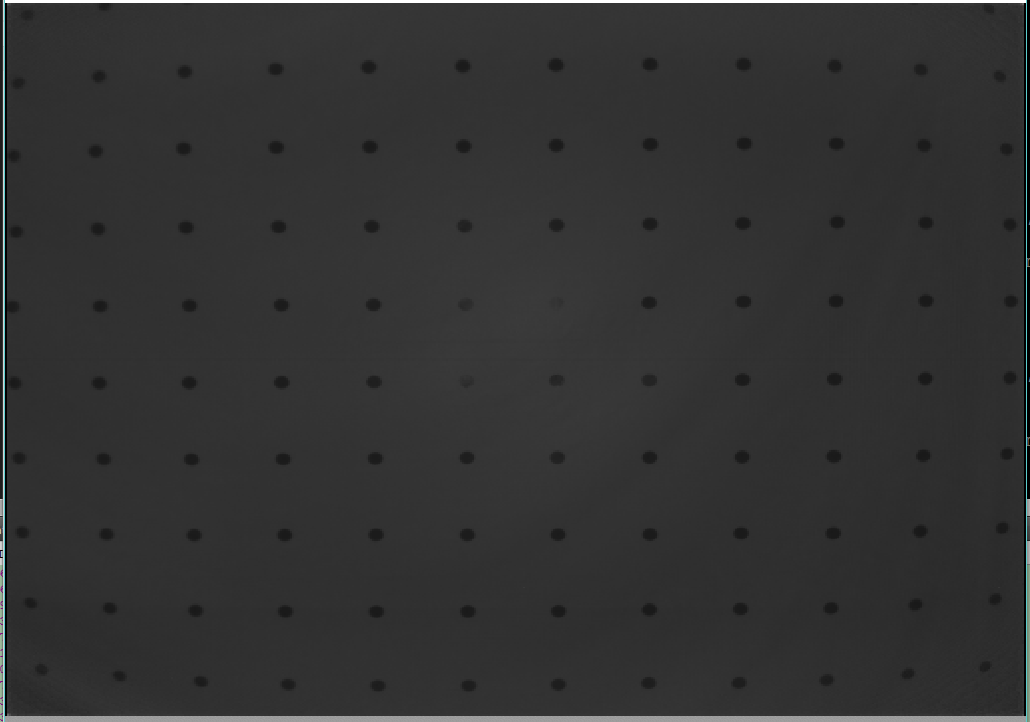
\includegraphics[width=0.5\textwidth]{Raw_Single_NIR}
%\label{Raw_Single_NIR}}
%\subfloat[Histogram Equalized \gls{NearIR}][Histogram Equalized]{
%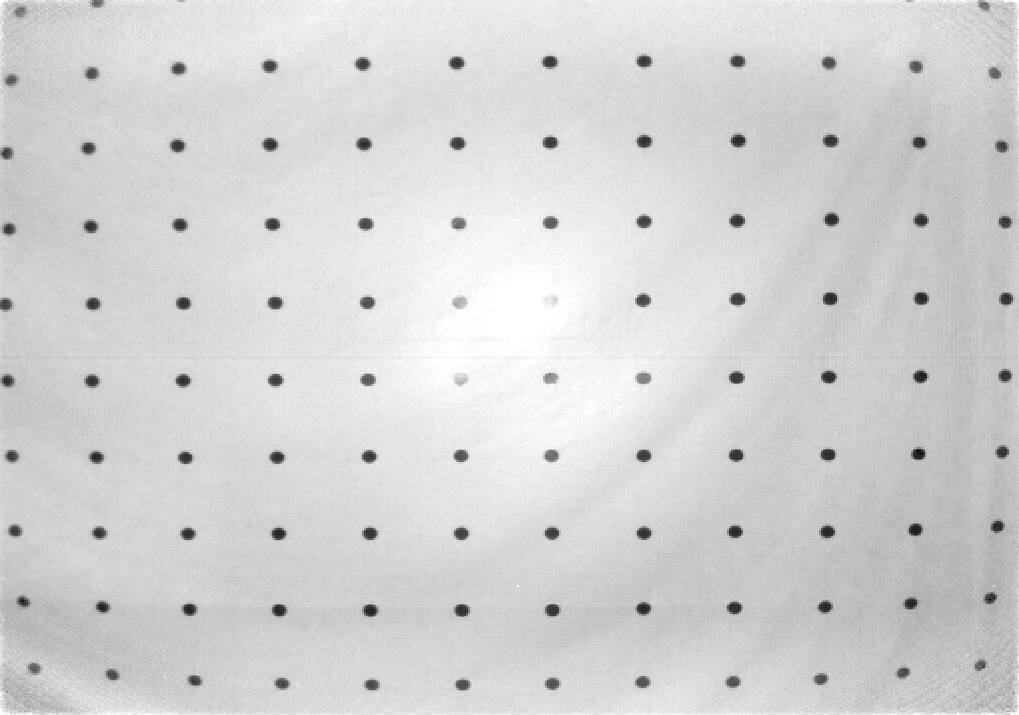
\includegraphics[width = 0.5\textwidth]{NIR_After_HistogramEqualization}
%\label{NIR_After_HistogramEqualization}}
%%\qquad
%\caption{\gls{NearIR} Streams before / after Histogram Equalization}
%\label{Histogram_Equalization}
%\end{figure}%
%%
%Commonly, Probability Mass Function (PMF) and Cumulative Distributive Function (CDF) will be calculated to determine the minimum valid intensity value (\(floor\)) and maximum valid value (\(ceiling\)) for rescaling, whereas tricks could be used by taking advantage of the \gls{GPU} drawing properties.%
%\\\indent%
%PMF means the frequency of every valid intensity value for all of the pixels in an image. Dividing all of the pixels in terms of their intensity values into \(N\) levels, every pixel belongs to one level of them, which is called gray level. With an proper selection of \(N\) to make sure a good accuracy, the intensity value of a pixel could be expressed based on its gray level \(n\)
%%
%\begin{equation}
%Intensity = n/N * (1 - 0) + 0 = n/N \, ,
%\end{equation}%
%\noindent
%where \(n\) and \(N\) are integers and \(1 \leqslant n \leqslant N\).%
%%
%PMF calculation is very similar with the points-drawing process in terms of \gls{GPU} that, both of them share the properties of pixel-by-pixel calculation. For the \gls{GPU} points-drawing process onto a customer framebuffer, the single-floating \enquote{color} value could go beyond the normal range [0, 1], with a maximum value of a signed 32-bit integer (\(2^{31}\) - 1). And different \enquote{color} values will be added together to form a \enquote{summational-color} in the case that some pixels are drawn onto the same position coordinates. \enquote{Taking} the range of pixel intensity values [0, 1] \enquote{as} a segment on x-axis waiting to be drawn, the intensity frequency \enquote{as} the \enquote{summational-color} of multiple pixels with different intensity drawn at the same position, and the counting process of intensity frequency \enquote{as} a points-drawing process, PMF could be calculated by drawing all of the pixels onto the x-axis within the normal intensity range [0, 1], with every single pixel's position coordinates re-assigned as (\(pixel\_intensity\), \(0\)) and its \enquote{color} value constantly being equal to one. Given the width (range of x-axis) of customer framebuffer being [-1, 1] in OpenGL, which is twice the range of pixel intensity [0, 1], the half-width of the customer framebuffer is same with the total number \(N\) of gray levels, which determines the precision of \(floor\) / \(ceiling\) intensity selection. 
%\\\indent%
%With PMF calculated and each intensity frequency that mapped to its corresponding gray level saved in the customer framebuffer, CDF could be easily calculated as
%%
%\begin{equation}
%%
%CDF(n) = \frac{sum}{N_{\text{\_Total Pixels/Image}}} \, ,
%%\label{lensDistortion}
%%
%\end{equation}%
%%
%where the gray level \(n\) is counted from the middle of the framebuffer's width to the end (1 \texttildelow \, \(N\)). And \(sum\) is the summation of customer framebuffer's values added up consecutively from 1 till \(n\). %
%%
%Then, at appropriate CDFs, e.g., \(CDF(n_{\text{\_floor}}) = 0.01\) and \(CDF(n_{\text{\_ceiling}}) = 0.99\), the intensities \(floor\) and \(ceiling\) could be written as
%%
%\begin{equation}
%\begin{aligned}
%floor &=  n_{\text{\_floor}} / N%
%\\%
%ceiling &=  n_{\text{\_ceiling}} / N
%\end{aligned}
%\label{intensityFloorCeilingDetermination}
%\end{equation}%
%%
%\noindent
%Finally, a new intensity value of every single pixel in an image could be rescaled as
%%
%\begin{equation}
%Intensity_{\text{\_new}} = \frac{Intensity_{\text{\_original}} - floor}{ceiling - floor} 
%\end{equation}%
%%
%\noindent
%After this final rescaling step of Histogram Equalization, the new image gets better contrast effect, as shown in Fig.~\ref{NIR_After_HistogramEqualization}%
%\\\\\indent%
%%% Adaptive Thresholding
%Affected by radial dominated lens distortions, the intensity value tend to decrease as the position of a pixel moves from the center of an image to the borders, in the case of observing a singular color view. Therefore, an adaptive thresholding process is needed, whereas using fixed thresholding will generate too much noise around borders. To segment the black dots from white background, we could simply subtract an image's background from an textured image, where the background comes from a blurring process of that image.%
%%
% \begin{figure}[t]
%\hspace*{-0.5cm}
%\centering
%\subfloat[Histogram Equalized \gls{NearIR}][Histogram Equalized]{
%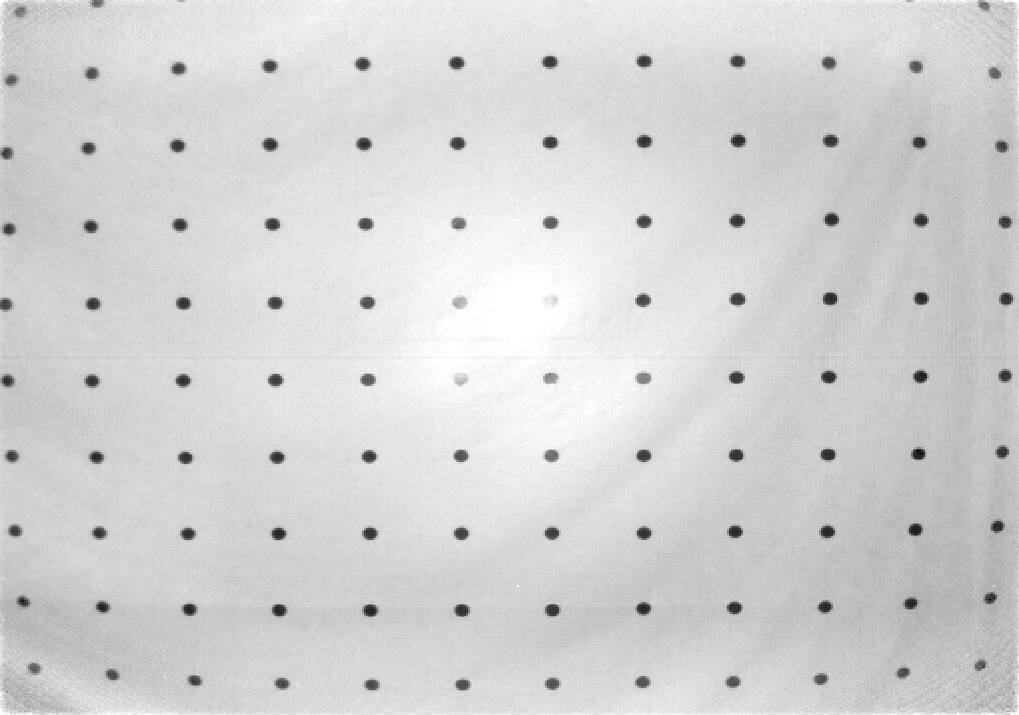
\includegraphics[width = 0.5\textwidth]{NIR_After_HistogramEqualization}
%\label{NIR_After_HistogramEqualization}}
%\subfloat[After Adaptive Thresholding][Binarized]{
%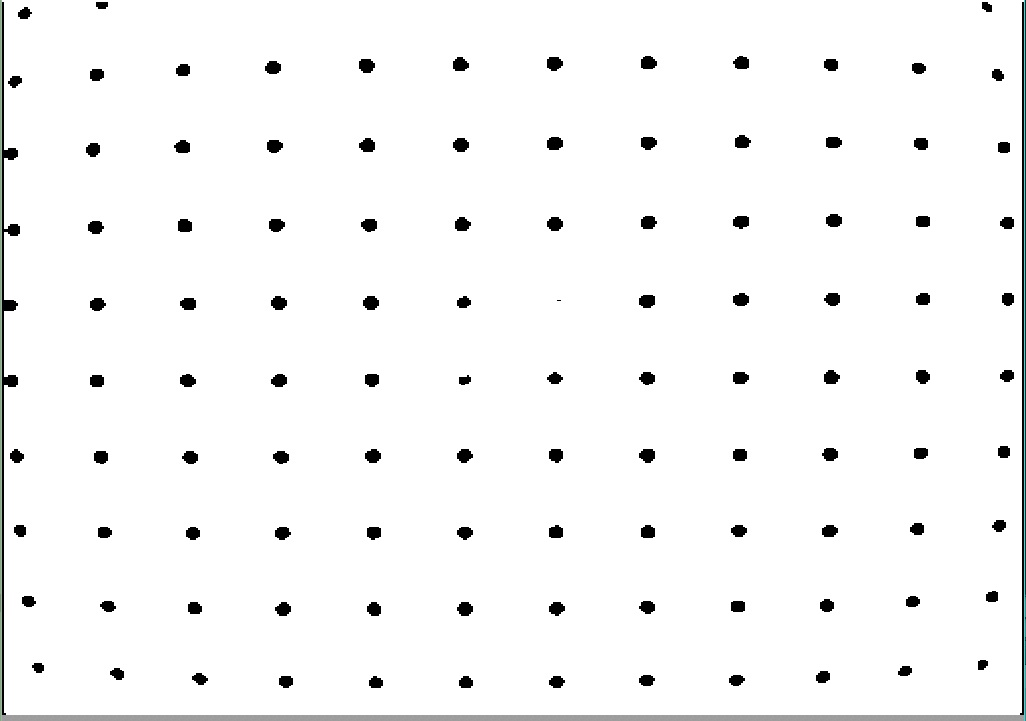
\includegraphics[width=0.5\textwidth]{Binarized_Single_NIR}
%\label{Binarized_Single_NIR}}%\qquad
%\caption{\gls{NearIR} Streams before / after Adaptive Thresholding}
%\label{Adaptive_Thresholding}
%\end{figure}%
%%
%There are three common types of blurring filters: mean filter, weighted average filter, and gaussian filter. Mean filter is selected for this background-aimed blurring process, because it has the smallest calculation and also a better effect of averaging than the others. After the blurred image containing background information is obtained, the binarizing (subtraction) process for every single pixel could be written as
%
%\begin{equation}
%%
%Intensity_{\text{\_binarized}} = %
%%
%\begin{cases}
%\,\, 1 , \quad \quad I_{\text{\_textured}} - I_{\text{\_background}}  -  C_{\text{\_offset}} \,\, > \,\,0 %
%\\%
%\,\, 0 , \quad \quad \quad \quad else%
%\end{cases}
% \, ,%
%\end{equation}%
%%
%where \(I\) is short for \(Intensity\) of every single pixel, and \(C_{\text{\_offset}}\) is a small constant that could be adjusted depending on various thresholding situations. In this project, \(C_{\text{\_offset}}\) is around 0.1.%
%%
%To sharpen the edge of the binarized image for a better \enquote{circle} shape detection, a median filter could be added as the last step of adaptive thresholding. As shown in Fig.~\ref{Adaptive_Thresholding}, background is removed in the binarized image after adaptive thresholding.
%\\\indent
%%
%%
%% Sniffer for Round Dot Center
%After the adaptive thresholding, image data saved on \gls{GPU} is now composed of circle-shaped \enquote{0}s within a background of \enquote{1}s. In order to locate the center of those \enquote{0}s circle, which is the center of captured round dot, it is necessary to know the edge of those circles. A trick is used to turn all of the edge data into markers that could lead a pathfinder to retrieve circle information.%
%%
%The idea that helps to mark edge data is to reassign pixels' values (intensity values) based on their surroundings. Using letter \(O\) to represent one single pixel in the center of a $3\times3$ pixels environment, and letters from \(A\)\texttildelow \(H\) to represent surroundings, a mask of 9 cells for pixel value reassignment could be expressed as below.
%
%\begin{center}
%  \begin{tabular}{ | c | c | c | }
%    \hline
%    \(E\) & \(A\) & \(F\) \\ \hline
%    \(B\) & \(O\) & \(C\) \\ \hline
%    \(G\) & \(\gls{D}\) & \(H\) \\
%    \hline
%  \end{tabular}
%\end{center}
%%
%To turn the surroundings \(A\)\texttildelow \(H\) into marks, different weights will be assigned to them. Those markers with different weights have to be non-zero data, and should be counted as the edge-part of circles. Therefore, the first step is to inverse the binary image, generating an image that consists of circle-shaped \enquote{1}s distributed in a background of \enquote{0}s.%
%%
%After reversing, the next step is to assign weight to the surroundings. OpenGL offers convenient automatic data type conversion, which means the intensity values from \enquote{0} to \enquote{1} of single-floating data type save on \gls{GPU} could be retrieved to CPU as unsigned-byte data type from \enquote{0} to \enquote{255}. Considering a bitwise employment of markers, a binary calculation related weight assignment is used in the shader process for pixels. The intensity reassignment for every single pixel is expressed as the equation below.
%%
%\begin{equation}
%\hspace*{-0.1cm}%
%%
%I_{\text{\_Path Marked}} = I_{\text{\_Original}} * \frac{(128I_{\text{A}} + 64I_{\text{B}} + 32I_{\text{C}} + 16I_{\text{\gls{D}}} + 8I_{\text{E}} +  4I_{\text{F}} +  2I_{\text{G}}+I_{\text{H}})}{ 255 }
%%
%\label{snifferDistributionWeight}
%\end{equation}%
%\indent%
%After this reassignment, the image is not binary any more. Every non-zero intensity value contains marked information of its surroundings, data at the edge of circles are now turned into fractions. In other words, the image data saved on \gls{GPU} at the moment is composed of \enquote{0}s as background and \enquote{non-zero}s circles, which contains fractions at the edge and \enquote{1}s in the center.%
%%
%Now, it is time to discover dots through an inspection over the whole path-marked image, row by row and pixel by pixel. Considering that, a process of one single pixel in this step may affect the processes of the other pixels (which cannot be a parallel processing), it is necessary to do it on CPU. The single-floating image data will be retrieved from \gls{GPU} to a buffer on CPU as unsigned-byte data, waiting for inspection. And correspondingly the new CPU image will have its \enquote{non-zero}s circles composed of fractions at the edge and \enquote{1}s in the center. Whenever a non-zero value is traced, a dot-circle is discovered and a singular-dot analysis could start. The first non-zero pixel will be called as an anchor, which means the beginning of a singular-dot analysis. %
%%
%During the singular-dot analysis beginning from the anchor, very connected valid (non-zero) pixel will be a stop, and a \enquote{stops-address} queue buffer is used to save addresses of both visited pixels and the following pixels waiting to be visited. On very visit of a pixel, there is a checking procedure to find out valid (non-zero) or not. Once valid, the following two steps are waiting to go. The first step is to sniff, looking for possible non-zero pixels around as the following stops. And the second step is to colonize this pixel, concretely, changing the non-zero intensity value to zero. Every non-zero pixel might be checked 1\texttildelow 4 times, but will be used to sniff for only once.%
%\\\indent%
%As for the sniffing step, base on the distribution table of \(A\)\texttildelow \(H\) that has been discussed above and their corresponding weight given by equation \ref{snifferDistributionWeight}, the markers \(A\)/\(B\)/\(C\)/\(\gls{D}\) are valid (non-zero) as long as the intensity value of pixel \(O\) satisfies the following conditions shown as below.%
%%
%\begin{equation}
%%
%\begin{aligned}
%if \,\, ( I_{\text{O}} \,\, \& \,\, \text{0x80}  == 1 ),\quad &then, \quad \text{marker } A\,\, \text{is valid \,\,( go Up )}%
%\\%
%if \,\, ( I_{\text{O}} \,\, \& \,\, \text{0x40}  == 1 ),\quad &then, \quad \text{marker } B\,\, \text{is valid \,\,( go  Left)}%
%\\%
%if \,\, ( I_{\text{O}} \,\, \& \,\, \text{0x20}  == 1 ),\quad &then, \quad \text{marker } C\,\,\text{is valid \,\,( go Right )}%
%\\%
%if \,\, ( I_{\text{O}} \,\, \& \,\, \text{0x10}  == 1 ),\quad &then,\quad \text{marker } \gls{D}\,\,\text{is valid \,\,( go Down )}%
%\\%
%\end{aligned}
%%
%\end{equation}%
%%
%\noindent
%Once a valid marker is found, its address \((column, row)\) will be saved into the \enquote{stops-address} queue. One pixel's address might be saved for up to 4 times, but \enquote{colonizing} procedure will only happen once at the first time, so that the sniffing will stop once all of the connected valid pixels in a singular dot-cluster are colonized as zeros.%
%%
% \begin{figure}[t]
%\hspace*{-0.5cm}
%\centering
%\subfloat[After Adaptive Thresholding][before Extraction]{
%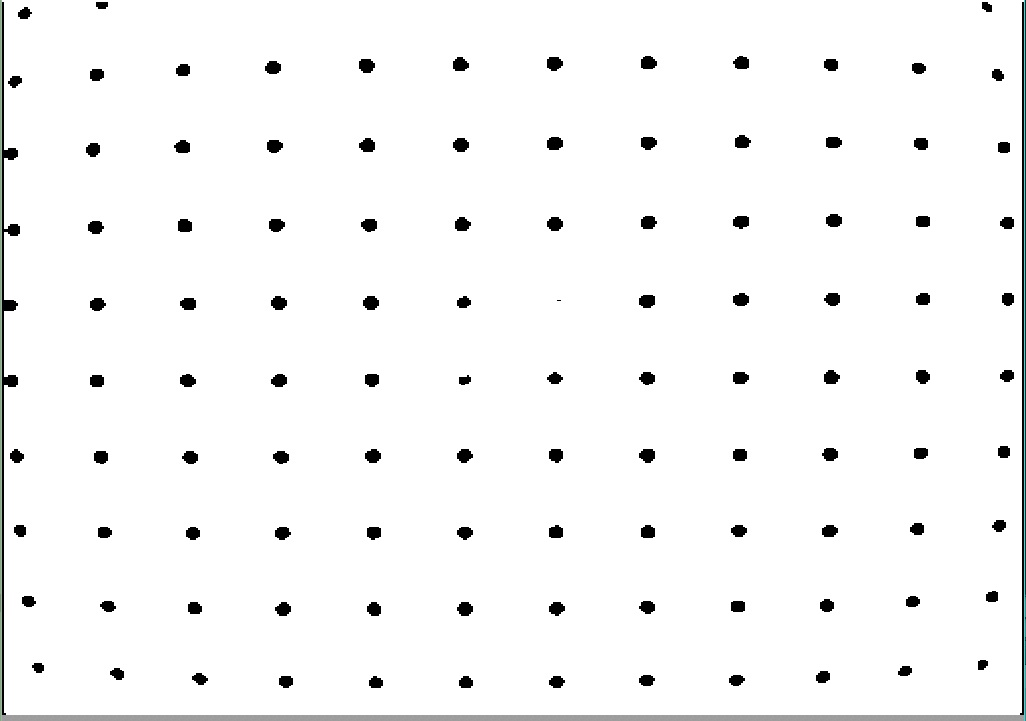
\includegraphics[width=0.5\textwidth]{Binarized_Single_NIR}
%\label{Binarized_Single_NIR}}
%%\qquad
%\subfloat[Dot Centers Extraction][Extracted and Marked]{
%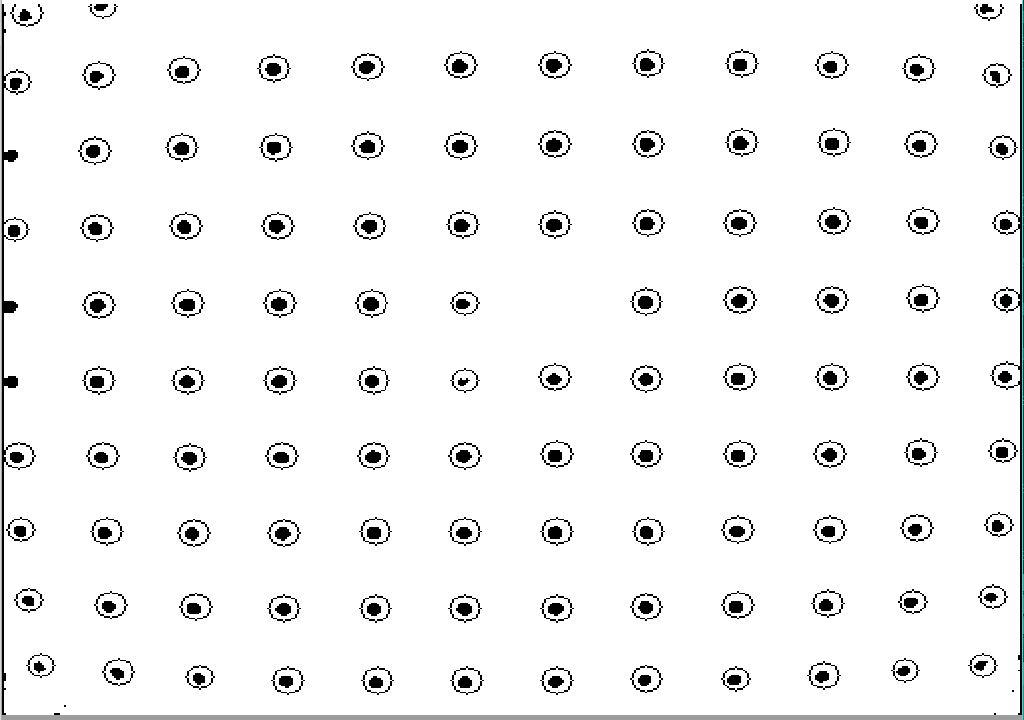
\includegraphics[width = 0.5\textwidth]{Dots_Extracted_Single_NIR}
%\label{Dots_Extracted_Single_NIR}}
%%
%\caption{Valid Dot-Clusters Extracted in \gls{NearIR}}
%\label{DotCentersExtraction}
%\end{figure}
%%
%In the second step \enquote{colonizing},  \(I_{\text{O}}\) is changed to zero, variable \(area\) of this dot-cluster pluses one, and bounding data \(RowMax\) / \(RoxMin\) / \(ColumnMax\) / \(ColumnMin\) are also updated.%
%%
%Finally, the Round Dot Centers \((column, row)\) could be determined as the center of bounding boxes with their borders \(RowMax\) / \(RoxMin\) / \(ColumnMax\) / \(ColumnMin\). After potential noises being removed based on their corresponding \(area\) and shape (ratio of width and height), the data left are taken as valid dot-clusters. As shown in Fig.~\ref{Dots_Extracted_Single_NIR}, the centers of valid dot-clusters are marked within their corresponding homocentric circles.
%\\\\%
%%
%%%\subsection{\((\gls{worldX}, \,\gls{worldY})\) Fitting based on Uniform Grid}
%%\label{uniformGridFittingXY}
%%%
%%The list of round dot centers \((column, row)\)s is extracted through section \ref{RowColumnExtraction}. The following is to map every dot center's \((column, row)\) to its corresponding world coordinates \((\gls{worldX}, \,\gls{worldY})\). As shown in Fig.~\ref{trackingModuleOnKinectV2CalibrationSystem}, world coordinates are from the uniform grid. Taking the side of unit-square (distance between two adjacent dots) as \enquote{Unit One} in the world coordinates and one dot as the origin of plan \(X^WY^W\), every dot cluster's center \(\gls{imageColumn}\) / \(\gls{imageRow}\) will be mapped to integer values \(\gls{worldX}\)/\(\gls{worldY}\). %
%%\\\\%
%%Ideally, a $3\times3$ perspective transformation matrix could help set a linear mapping between two plane coordinates, and 3 dot centers with know coordinates pair of \((column, row)\) and \((\gls{worldX}, \,\gls{worldY})\) are enough to determine the transformation matrix. Once four points with a squared-shape \(\gls{imageColumn}\)/\(\gls{imageRow}\) distribution is found, a $3\times3$ perspective transformation matrix \(A\) could be determined by solving eqn.~\ref{perspectiveDistortionCorrectionEquation}, %
%%where \(C\) and \(R\) are vectors consist of \((column, row)\)s of four squared-shape distributed points; \(\gls{worldX}\) and \(\gls{worldY}\) are vectors consist of four points \((0, 0)\), \((0, 1)\), \((1, 1)\), and \((1, 0)\); \(z\) denotes the third axis in the homogenous system connecting two planes. %
%%\\\\%
%%Due to the distortions, cluster centers in image plane are not uniformly distributed, and this $3\times3$ transformation matrix can only generate corresponding decimal \(\gls{worldX}\)/\(\gls{worldY}\) values that are close integers. But in practice, the correct integer values \(\gls{worldX}\)/\(\gls{worldY}\) could still be calculated through \(Rounding\). The list of cluster centers' image coordinate \((column, row)\)s can give many groups of four squared-shape distributed points, while each of them gives a different image coordinate distance that maps to the \enquote{Unit One} in world coordinates. Taking those points with generated \(\gls{worldX}\)/\(\gls{worldY}\) values that are within an appropriate range close to integers as valid points, the \enquote{best} $3\times3$ transformation matrix could be determined by going through all of the possible groups of four squared-shape distributed points and picking out the group that leads to the most valid points.%
%%\\\\%
%%In this way, the so-called \enquote{best} transformation matrix can give a best \enquote{Unit One} distance in image coordinate, however its corresponding origin point \((0, 0)\), one of the four points that are used to calculate a transformation matrix, is usually not close to the center of cameras' Field of View (\gls{FoV}). A translation matrix \(T\) could be used to refine the \enquote{best} transformation matrix, and help to translate the origin point to be a dot cluster that is closest to the center of \gls{FoV}. The refined transformation matrix \(A_{\text{\_refined}}\) is written as%
%%%
%%\begin{equation}
%%%
%%A_{\text{\_refined}}%
%%= %
%%T \cdot A %
%%= %
%%\begin{bmatrix} 
%%1 & 0 & -X_{\text{\_Zero\_A}} \\%
%%0 & 1 & -Y_{\text{\_Zero\_A}} \\%
%%0 & 0 &   1 \\%
%%\end{bmatrix}%
%%\cdot A%
%%%
%%\end{equation}%
%%%
%%where the integer world coordinate point \((X_{\text{\_Zero\_A}}, \, Y_{\text{\_Zero\_A}})\) are mapped from the center point \((C_{\text{\_center}}, \, R_{\text{\_center}})\) of \gls{FoV} in image plane by the so-called \enquote{best} transformation matrix \(A\), written as%
%%%
%%\begin{equation}
%%%
%%\left[ \begin{array}{c} %
%%zX_{\text{\_Zero\_A}} \\ zY_{\text{\_Zero\_A}} \\ z \end{array} \right] %
%%= %
%%A\cdot \left[ \begin{array}{c} %
%%C_{\text{\_center}} \\ R_{\text{\_center}} \\ 1 \end{array} \right] %
%%%
%%\end{equation}%
%%%
%%Eventually, the refined transformation matrix eventually generates a list of world coordinate points \((\gls{worldX}, \, \gls{worldY})\)s that correspond to image coordinates \((column, row)\)s. As shown in Fig.~\ref{XY_GridFitting_Matlab}, world coordinates are integers and the origin (blue circle) is chosen as where the center-closest dot-cluster is sitting.\par%
%%%
%% \begin{figure}[t]
%%\hspace*{-0.3cm}
%%\centering
%%\subfloat[Image Plane Coordinates][ImagePlane Coordinate]{
%%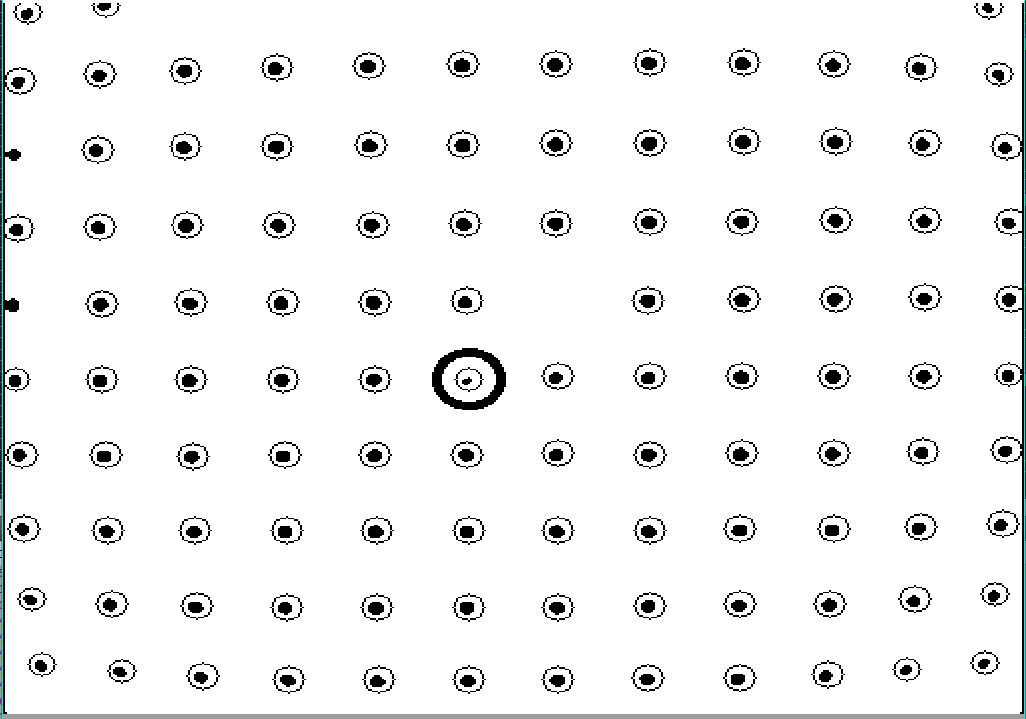
\includegraphics[width=0.54\textwidth, height = 0.425\textwidth]{Grid_Centered_Single_NIR}
%%\label{Grid_Centered_Single_NIR}}
%%%\qquad
%%\subfloat[World Coordinates][World Coordinate]{
%%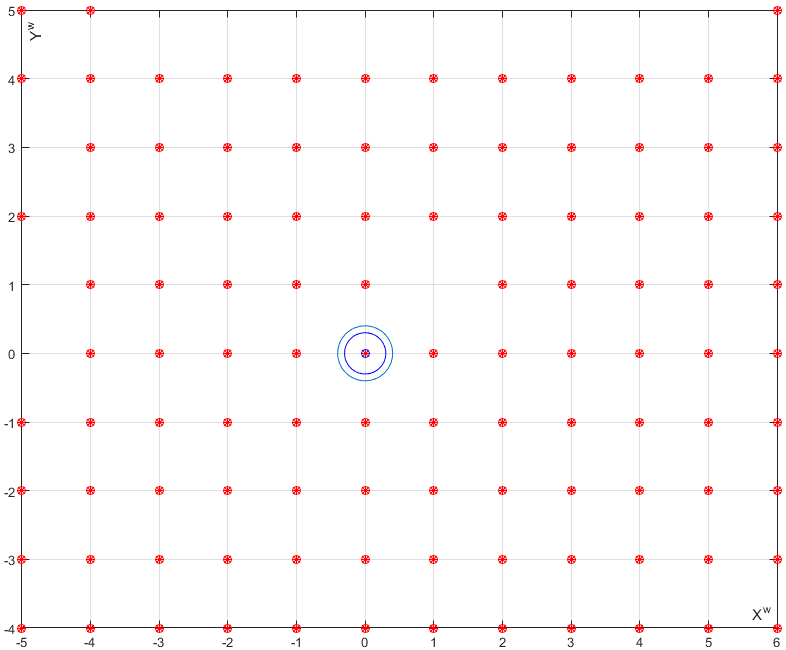
\includegraphics[width = 0.47\textwidth, height = 0.425\textwidth]{XY_GridFitting_Matlab}
%%\label{XY_GridFitting_Matlab}}
%%%
%%\caption{Coordinates-Pairs: (Row, Column)s and (\(\gls{worldX}\), \(\gls{worldY}\))s}
%%\label{Grid_Fitting}
%%\end{figure}%
%%
%%
%%\subsection{Mathematical tools}
%%\subsubsection{Singular Value Decomposition (SVD)}
%%\subsubsection{Least Square with Pseudo-Inverse}
%%
%\section{Alignment of RGB Pixel to Depth Pixel}
%A undistorted \gls{3D} reconstruction could be displayed with the help of a \gls{LUT} generated by the per-pixel calibration method, which has been discussed in section~\ref{sectionPerPixelCalibration}. However, we have not figured out yet what the color of each pixel is. To generate a colored \gls{3D} reconstruction with a combination of a random depth sensor and a random RGB sensor, we need to align the RGB pixels to depth pixels. The intermediate between the depth sensor image space and RGB sensor image space is the world space. As long as we figure out the mapping from world space to RGB sensor image space, the color of pixel with known \(X^WY^WZ^W\) could be looked up from the RGB image space. The pinhole camera matrix \(M\) is used to map from world space to RGB image space. Using the frame data from Kinect RGB steams and Kinect \gls{NearIR} streams, a Matlab prototype of RGB pixels alignment is shown in Fig.~\ref{RGBAligned_Matlab}, where the RGB textured is mapped onto its corresponding \gls{NearIR} image, who has same pixels with depth sensor. The total black area on the top edge and bottom edge is where the depth sensor's view goes beyond the RGB sensor's view. Fig.~\ref{RGBAligned_Qt} shows the screen-shot of live video after calibration with the RGB pixels aligned by a pinhole camera model \(M\).
%
%%
% \begin{figure}[b]
%\hspace*{-0.5cm}
%\centering
%\subfloat[][]{
%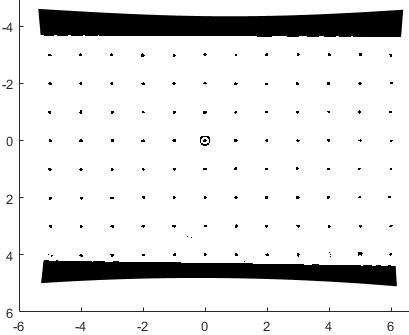
\includegraphics[width = 0.5\textwidth]{RGBAligned_Matlab}
%\label{RGBAligned_Matlab}}
%\subfloat[][]{
%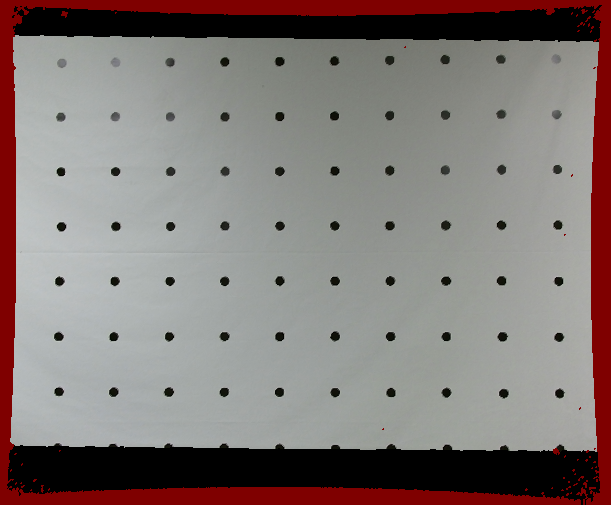
\includegraphics[width=0.5\textwidth]{RGBAligned_Qt}
%\label{RGBAligned_Qt}}
%\caption{Alignment of RGB Texture onto \gls{NearIR} Image}
%\label{Adaptive_Thresholding}
%\end{figure}%
%%
%
%\section{Summation}
%A per-pixel calibration method, using a moving plane calibration system, is proposed in this chapter. The main idea of this calibration method is to make it available to generate accurate (undistorted) per-pixel world space position (\(\gls{worldX}, \, \gls{worldY}, \, \gls{worldZ}\)) directly in real-time with the fewest calculation. The per-pixel \(\gls{worldZ}\) will be mapped from per-pixel depth value \(\gls{D}\), and then per-pixel \(\gls{worldX}/\gls{worldY}\) will be determined by per-pixel linear beam equation from its corresponding \(\gls{worldZ}\). Note that the per-pixel beam equation represents the lens-distortion removed field of view of a single pixel. And the \enquote{depth distortion} could be removed during the per-pixel mapping from \(\gls{D}\) to \(\gls{worldZ}\). In short, this per-pixel calibration method consists of two big steps: \(X^WY^WZ^W+\gls{D}\) data collection and mapping parameters determination. \(\gls{D}\) is simply from depth streams. \(\gls{worldZ}\) is from external based on the camera's position on the rail. And the undistorted (\(\gls{worldX}, \, \gls{worldY}\)) are from the transformation of \(R/C\) by a \(4^{th}\) order polynomial mapping model, during which lens-distortions could be removed. With the frames data of \(X^WY^WZ^W+\gls{D}\) collected, the per-pixel mapping parameters \(a/b/c/d/e/f\) could be determined by eqn.~\ref{fromD_To_Z} and eqn.~\ref{kaiBeamEquation}. 
%\\\indent
%Without using the traditional pinhole camera model, two polynomial mapping models are employed in this calibration method. The first model is the two-dimensional \(4^{th}\) order polynomial mapping from \(R/C\) to \(\gls{worldX}/\gls{worldY}\) during the frames data collection, which takes care of the removal of lens distortions; and the second model is the linear mapping from \(\gls{D}\) to \(\gls{worldZ}\), which can handle \enquote{depth distortion}. Both of the two mapping models are determined and calculated by real streams data from the camera, so that we claim this per-pixel calibration method a \enquote{data-based} calibration method. 
%\\\indent
%Besides the data-based calibration method, a robust \gls{DIP} process during calibration is also discussed, which guarantees that the live video during undistorted frames collection could be in real-time. Note that \enquote{real-time} here means being able to show an undistorted frame before the start of the second frame processing. After the undistorted \gls{3D} reconstruction, the alignment of the RGB pixel to Depth pixel is also discussed. The data-based calibration method could be applied universally on any \gls{RGBD} cameras. With the alignment of RGB pixels, it could even work on the combined \gls{3D} camera of a random Depth sensor and a random RGB sensor.
%
%
%
%
%
%
%
%
%
%
%
%
%
%
%
%
%
%
%











